\documentclass[
	%parspace, % Add vertical space between paragraphs
	%noindent, % No indentation of first lines in each paragraph
	%nohyp, % No hyphenation of words
	%twoside, % Double sided format
	%draft, % Quicker draft compilation without rendering images
	%final, % Set final to hide todos
]{elteikthesis}[2024/04/26]

% \pdfobjcompresslevel=0 % Disable object compression

% The minted package is also supported for source highlighting
% See elteikthesis_minted.tex for example
%\usepackage[newfloat]{minted}

% Document's metadata
\title{LiDAR Odometry and Mapping\\Beyond RTK Accuracy } % title
\date{2025} % year of defense

% Author's metadata
\author{Liviu-Daniel Florescu}
\degreetitle{MSc Intelligent Field Robotic Systems (IFRoS)}

% Superivsor(s)' metadata
\supervisor{Iván Eichhardt} % internal supervisor's name
\affiliation{Assistant Professor} % internal supervisor's affiliation
\extsupervisor{Maximilian Fenkart} % external supervisor's name
\extaffiliation{CTO, Sodex Innovations GmbH} % external supervisor's affiliation

% University's metadata
\university{Eötvös Loránd University} % university's name
\faculty{Faculty of Informatics} % faculty's name
\department{Erasmus Mundus Joint Master in \\Intelligent Field Robotic Systems} % department's name
\city{Budapest} % city
\logo{elte_cimer_szines} % logo

% Add bibliography file
\addbibresource{bibliography.bib}

\makeglossaries

\newglossaryentry{surveying}
{
    name=surveying,
    description={The work of examining and recording the area and features of a piece of land in order to construct a map, plan, or detailed description thereof}
}

\newglossaryentry{pointcloud}
{
    name={point cloud},
    description={A set of point coordinates obtained as the output of a scanning sensor}
}

\newglossaryentry{fieldrob}
{
    name={Field Robotics},
    description={The area of robotics that focuses on robots operating in unstructured outdoor environments for tasks like agriculture or exploration}
}

\newglossaryentry{registration}
{
    name={registration},
    description={The process of aligning multiple point clouds in a single coordinate system such that matching features are as close as possible}
}

\newglossaryentry{odometry}
{
name={odometry},
    description={The process of computing relative displacement of a robot using on-board sensors}
}

\newglossaryentry{sfm}{
    name={Structure from Motion (SfM)},
    description={The task of reconstructing a 3D scene and a sequence of camera poses from a set of images}
}

\newglossaryentry{kdtree}{
    name={k-d tree},
    description={A data structure for organizing entries in a $k$-dimensional space using a tree structure. When $k$ is not very large, it provides logarithmic look-up time.}
}

\newglossaryentry{voxel}{
    name={voxel},
    description={A cuboid-shaped region in 3D space; a 3D cell.}
}

\newglossaryentry{keyframe}{
    name={keyframe},
    description={An image frame or 3D scan that is used for odometry estimation. Because modern sensors usually operate at higher frequencies than needed for most algorithms, it is a reasonable decision to skip frames based on a predefined pattern or condition, without sacrificing accuracy.}
}

\newacronym{lidar}{LiDAR}{Light Detection and Ranging}
\newacronym{slam}{SLAM}{Simultaneous Localization and Mapping}
\newacronym{ins}{INS}{Inertial Navigation System}
\newacronym{gnss}{GNSS}{Global Navigation Satellite System}
\newacronym{rtk}{RTK}{Real-Time Kinematics}
\newacronym{kf}{KF}{Kalman Filter}
\newacronym{ekf}{EKF}{Extended Kalman Filter}
\newacronym{pf}{PF}{Particle Filter}
\newacronym{icp}{ICP}{Iterative Closest Point}
\newacronym{ndt}{NDT}{Normal Distributions Transform}
\newacronym{loam}{LOAM}{LiDAR Odometry and Mapping}
\newacronym{lio}{LIO}{LiDAR-Inertial Odometry}
\newacronym{cnn}{CNN}{Convolutional Neural Network}



% The document
\begin{document}

% Set document language
\documentlang{english}

% List of todos (not in the final document)
%\listoftodos[\todolabel]

% Custom commands

\newcommand{\reffig}[1]{(Fig. \ref{fig:#1})}
\newcommand{\refch}[1]{(Chapter \ref{ch:#1})}



% Title page (mandatory)
\maketitle
% Topic declaration page (mandatory) - can also be attached instead

\includepdf[pages={2,3}]{other/TDF_liviu_florescu.pdf}

% Table of contents (mandatory)
\tableofcontents
\cleardoublepage

% Main content
\chapter{Introduction}
\label{ch:intro}

% - General description of robotics;
% - General description of perception;
% - General description of localization.

Like many scientific terms that we encounter in our daily activities, \emph{robotics} describes a broad collection of technologies and stands at the intersection of key research directions. Motivated by practicality, disciplines that appear completely unrelated find themselves building upon advancements in other fields, diluting boundaries and joining forces to enable otherwise-impossible advancements.

What constitutes a \emph{robot}, then? In its inceptive use by Karel Čapek \cite{roberts_robotics_history_1999} in 1921, the word stemmed from the Slavic \emph{robota}, meaning ``servitude'' or ``forced work'', and referred to a human-like mechanical system working on factory assembly lines. This concept, however, dates from earlier centuries. Around 1495, Leonardo Da Vinci envisioned a mechanical knight controlled by a series of pulleys, that was able to perform simple movements \cite{taddei_leonardo_robots_2008}. Testifying to the industrial revolution and the computational breakthroughs of the last few decades, modern-day humanoid robots can perform acrobatics \cite{bostondynamics_backflips_2023}, interact with humans in constrained scenarios \cite{humanoids_hospital} \cite{humanoid_school} \cite{humanoid_school2} and even replicate human facial expressions \cite{humanoid_facial}. Still, a device ought not necessarily appear human-like in order for it to be labeled as a robot. Autonomous vacuum cleaners, space rovers or crop-monitoring drones fall under the same category. At this stage, a complete taxonomy would have to address dozens of physical (size, shape, mobility, locomotion system, etc.) and non-physical (autonomy, perception abilities, use-case, etc.) characteristics, and none of these would independently convey the meaning that we intuitively associate to the notion of \emph{robot}. Without assessing whether an exhaustive, generic definition is even possible, we can synthesize the above by affirming that a \emph{robot} is an artificial system that performs one or more tasks and is able to evaluate its state or gather information from its environment.

\section{Robotic perception}

This formulation highlights two essential aspects of a robotic agent \reffig{robot-env}: actuation, seen as some form of dynamic physical ability, allowing the agent to enact the desired behavior, and perception, the ability to observe changes in the environment.

% Certainly, this  obfuscates several other key elements, such as control mechanisms, information management or a reasoning model, but it emphasizes the importance of perception as a vital link with the physical world. Additionally, this closely resembles the behavior model of humans, where sensing also plays a critical role.

\begin{figure}[H]
    \centering
    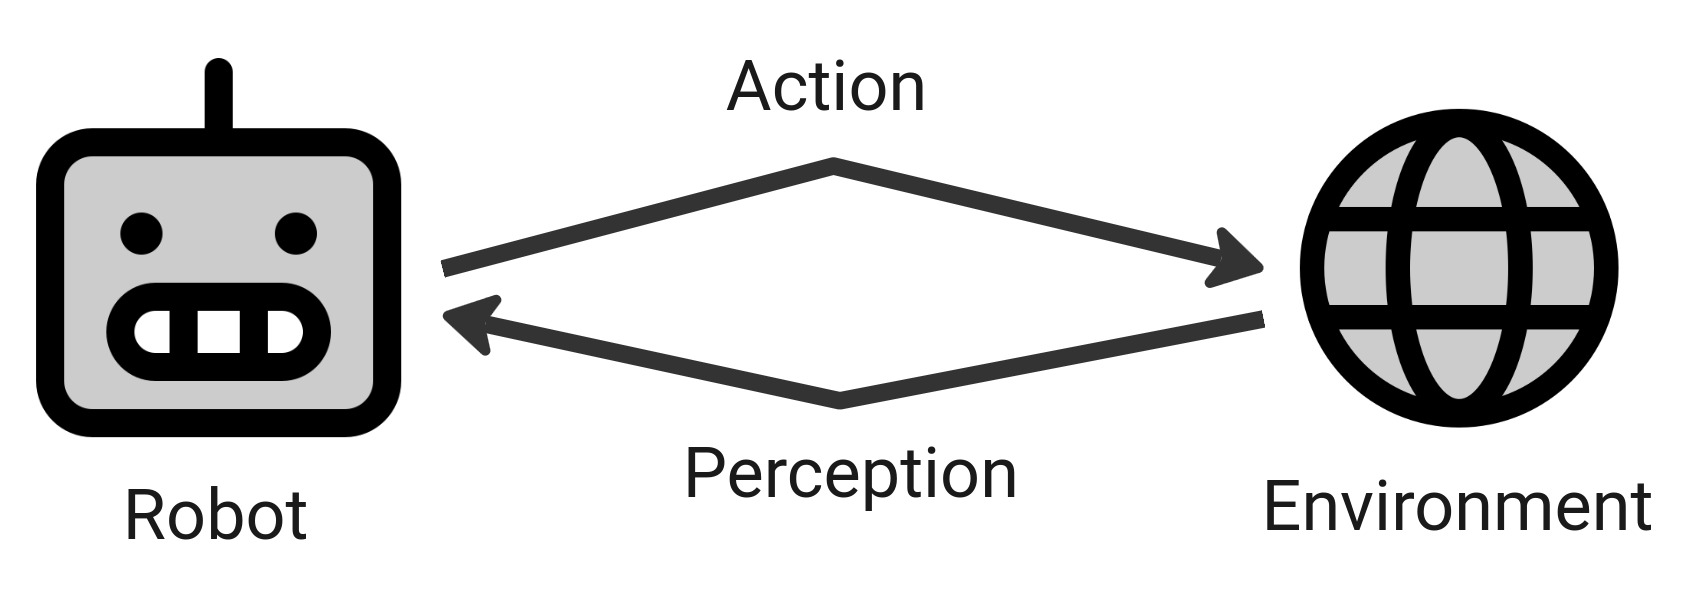
\includegraphics[width=0.6\linewidth]{robot-env.jpg}
    \caption[Perception in the Robot-Environment exchange]{A simplified interpretation of the robotics paradigm. The interaction between an agent and its environment can be seen as a two-way flow: the agent alters the environment through its actions, and uses perception to observe it.}
    \label{fig:robot-env}
\end{figure}

% Just as the human senses span multiple stimulus modalities, so does artificial perception, through the use of different types of sensors. An initial categorization differentiates between proprioceptive and exteroceptive sensors. The first type refers to sensors that provide information about the internal state of the system (virtually independent from the environment), while the second type consists of sensors that collect data about the world. Another division classifies sensors as active (emitting some form of energy in order to obtain a reading) or passive (which simply react to external stimuli).

Sensing modalities have largely different contributions to the perception mechanism. To this extent, the phrase \emph{visual dominance} was introduced by F. Colavita \cite{colavita1974human}, whose study demonstrated that humans focus more on the visual component when presented with an audiovisual stimulus, and following research has strongly confirmed this tendency \cite{Hutmacher2019} \cite{hecht2009sensory}. Unsurprisingly, a similar pattern is emerging in the case of robots, thanks to the reduced cost, familiarity and wide availability of cameras. In many situations, visual stimuli provide most of the necessary information, and this has motivated the development of various image processing algorithms.

Technological innovation in the last century has led to the situation in which artificial sensors surpass humans in both the range of signals that are perceived, as well as the accuracy of the measurements. A relevant example is the class of \acrfull{lidar} sensors which retrieve three-dimensional information about the environment at a very high frequency and with rather negligible measurement errors, in the form of \emph{\glspl{pointcloud}} \reffig{pcd-example}. Among many applications, this type of sensors can be used to construct virtual representations of a specific environment, enabling engineers to experiment with a realistic model, evaluate construction progress or validate a finished project.

\begin{figure}[H]
    \centering
    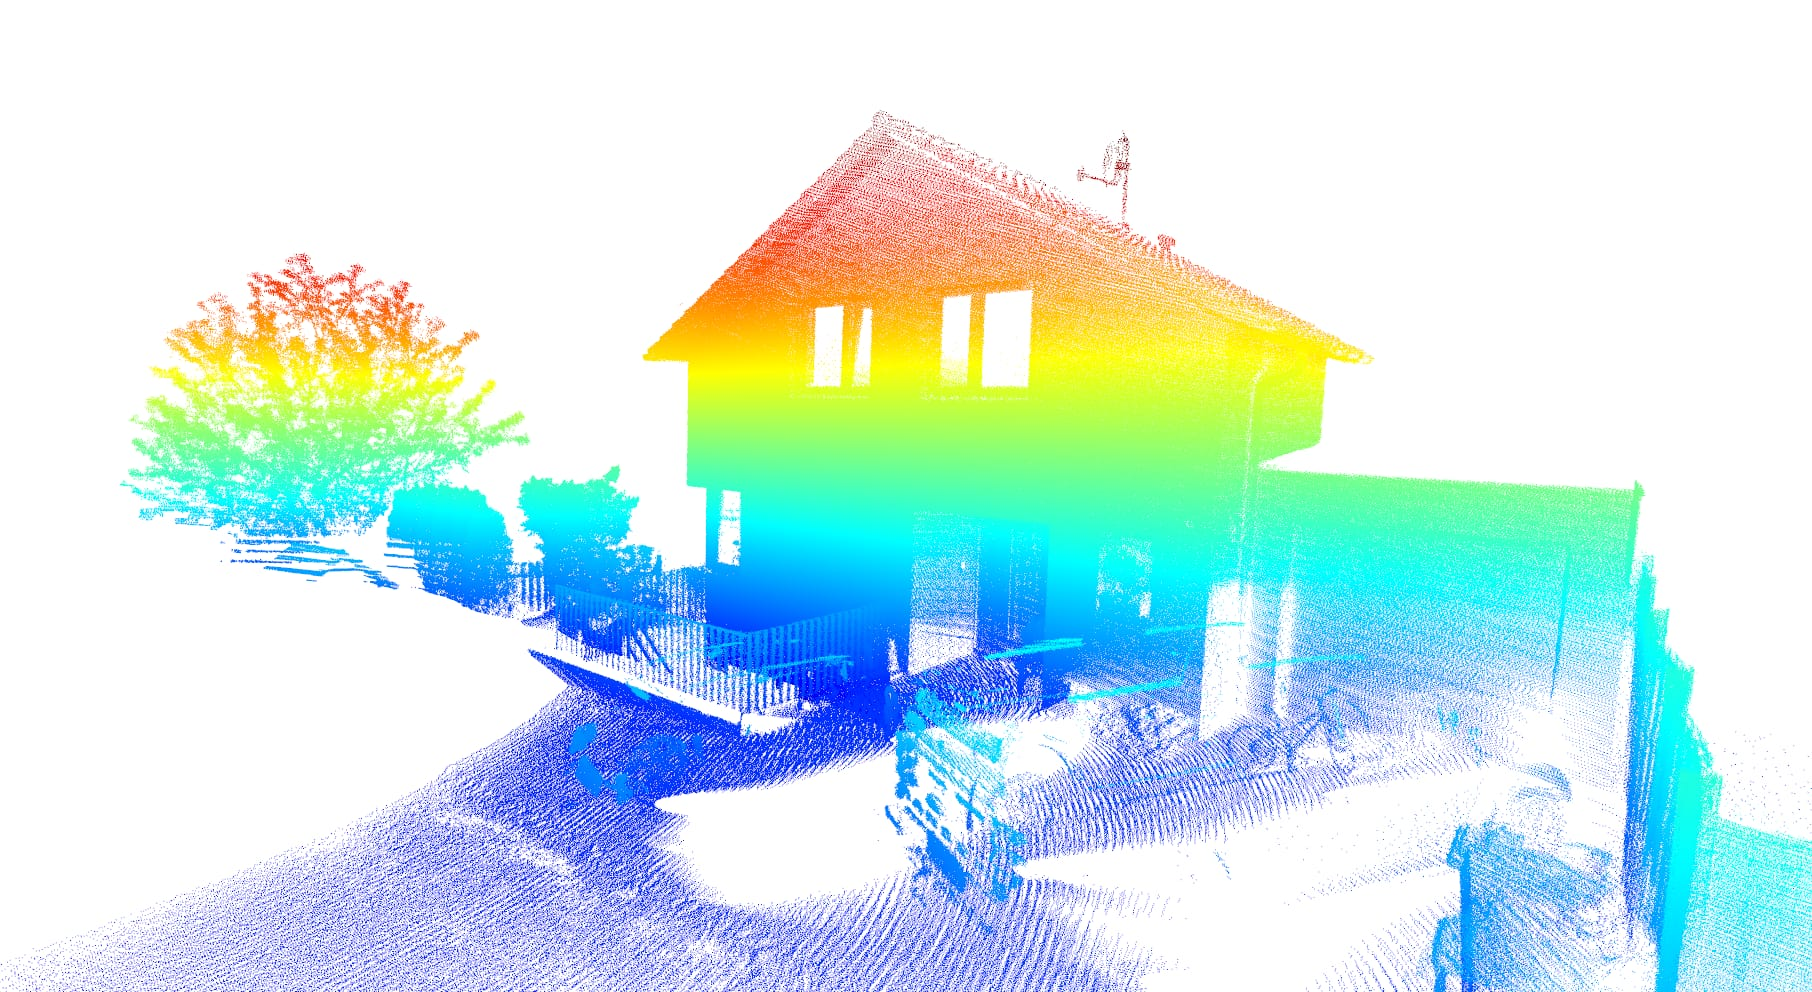
\includegraphics[width=0.7\linewidth]{images/pointcloud_example.jpeg}
    \caption[Point Cloud Example]{An example point cloud (points are colored by height), capturing the 3D representation of an outdoor scene. Multiple individual scans are placed into the same coordinate system to obtain a dense spatial representation.}
    \label{fig:pcd-example}
\end{figure}

\section{Problem definition}

The current work addresses a common and well-known problem in the area of \gls{fieldrob}, namely \acrfull{slam}, and combines the practicality of an industrial solution with a perception-based approach.

SDX-Compact \reffig{sdx-compact} is the main product of Sodex Innovations GmbH, consisting of multiple sensors that collect spatial and visual data. This module can be easily mounted on an arbitrary vehicle in order to expand its perception capabilities and convert it into a \gls{surveying} device. While the vehicle is moving, the LiDAR sensor captures 3D scans of the surroundings, as well as related metadata (timestamps, localization information, signal intensity etc.). Because the rig includes a high-accuracy \acrfull{ins}, the localization and orientation data can be used to join the collected point clouds and create a global 3D map of the traversed space.

Nonetheless, this suffers from two main limitations:

\begin{compactitem}
    \item Reliance on unstable signal: internally, the INS depends on information from a \acrfull{gnss} receiver, which is limited to outdoor spaces and whose availability varies depending on weather conditions and surroundings (e.g. thick vegetation, tall buildings, bridges).
    \item Unsatisfactory accuracy: when merging point cloud data, positioning or localization errors introduce inconsistencies in the final 3D model, which hinders precise planning and construction.
\end{compactitem}

Our work aims to address these limitations by introducing a component that utilizes the information collected by the LiDAR sensor in conjunction with the existing data. Three research questions have been formulated to guide this process:

\begin{compactenum}
    \item What metrics exist for measuring the accuracy of point cloud \gls{registration}? In this context, registration refers to placing a pair of related point sets in a common reference frame.

    \item Can methods that use only visual information achieve higher quality point cloud registration (3D mapping) than merging based on \acrfull{rtk}? Usually, GNSS systems provide meter-level accuracy. In the current scenario, however, the system is corrected using Real-Time Kinematics, such that the expected error is at centimeter-level.

    \item To what extent is LiDAR-based \gls{odometry} an alternative to GNSS localization? Previous research indicates that the spatial information present in 3D point clouds could be used to compute the relative displacement between consecutive scans, resulting in the ability to estimate odometry (an essential component of robotic localization) without dedicated sensors such as wheel encoders or accelerometers.
\end{compactenum}

The main contribution of the project consists of developing an original framework for localization and mapping based on data collected with an industrial sensor rig. The results are more generic than if a particular physical robotic system were involved, and thus are relevant for virtually any robotic application with a similar setup.

The following chapters of this document will cover related research directions and efforts that our work builds upon \refch{review}, a detailed description of the components and algorithms involved in developing the project \refch{methodology}, an evaluation of the method based on its results \refch{results}, as well as a series of conclusions that were drawn from the overall process \refch{conclusion}.



\cleardoublepage

\chapter{Background and Literature Review}
\label{ch:review}

The goal of this chapter is to present the research context in which our project was conducted, by looking at common methods for each of the main components and highlighting those that inspired the current approach.

\section{Simultaneous Localization and Mapping (SLAM)}

SLAM constitutes a key research area in robotics, because it is a foundational building block for autonomous operation. This problem occurs when the robot does not have prior access to a map of the environment, so it must construct one while keeping track of its current position (\emph{online} SLAM). If the goal is to optimize the entire sequence of poses along the robot path, this is known as the \emph{full} SLAM problem. \cite{thrun}

Usually, the problem is discretized along the time dimension, such that at time $t$ we aim to compute the posterior function $p(x_t, M|z_{1:t}, u_{1:t})$, where $x_t$ is the current state, $M$ is the map, $z_{1:t}$ represents the set of measurements collected so far, and $u_{1:t}$ the control sequence. As each of these variables can have different concrete representations, depending on the task and the available sensors, a broad range of approaches have been proposed.

% KF and EKF
Aulinas et al. \cite{aulinas2008slam} note that the earliest methods rely on probabilistic models derived from the recursive Bayes rule, as such formulations can provide intuitive representations of the various noisy components involved in a robotic system. When employing the \acrfull{kf} \cite{Kalman1960} or its variations, the robot state, measurements and control inputs are modeled as multi-dimensional Gaussians, whose covariances describe the associated uncertainty. The algorithm alternates between \emph{predictions}, when the state is modified based on $u_t$, and \emph{updates}, when the prediction is evaluated against the latest observation $z_t$, and the state hypothesis is updated accordingly. The \acrfull{ekf} maintains this structure but can accommodate non-linearities in the displacement or measurement functions by using local linear approximations. Such methods have been successfully applied for indoor \cite{davisonEKF}, aerial \cite{luo2013uav}, and underwater \cite{palomer2019inspection} robots.

\acrfull{pf}, introduced by Del Moral \cite{del1997nonlinear}, is a probabilistic approach that relies on the Monte Carlo method. Instead of an analytical form, the uncertainty is accounted for by considering a large set of samples (representing potential states) and weighting them based on measurement likelihood. This has a higher computational cost than the standard KF methods, but is not affected by any linearization limitations. Nie et al. \cite{lcpf2020} implemented a LiDAR SLAM algorithm based on PF localization, albeit for 2D mapping.

Another large group of methods is represented by \emph{Visual SLAM}, when cameras are the main (and sometimes only) sensor used. As early as 1980, Moravec \cite{moravec1980obstacle} developed a robot capable of estimating its motion by matching features in images captured at discrete poses, in a stop-and-go fashion. In 2007, SLAM was being performed using a single handheld camera \cite{davison2007monoslam,klein2007parallel}, triggering a separation from the popular, offline, \gls{sfm} techniques. The solution is even more robust when a stereo system is available \cite{mei2011rslam}, as this helps avoid the geometrical limitations of monocular vision.

\section{Point cloud Registration}

Before discussing LiDAR-based approaches in more detail, let us review the task of point cloud registration. Given two sets of points $P, Q$ in arbitrary reference frames, representing (at least partially) the same scene, the goal is to find the transformation $\matx{T} \in \SE{3} $ (translation and rotation) that best aligns the points. This can be expressed as an optimization problem:

\begin{equation}\notag
    \underset{\matx{T}}{\operatorname{argmin}}\,J(\matx{T}P, Q)
\end{equation}

where $J$ is a custom cost function. The particular case where known point correspondences are provided has a closed-form solution \cite{arun1987leastsquares}, but the \acrfull{icp} algorithm \cite{besl1992method} removes this constraint by alternating between correspondence generation --- each point in $P$ is paired with its nearest neighbor from $Q$ --- and minimizing the point-pair distances. This approach is by far the most widespread, thanks to its simplicity, computational efficiency (\eg using a \gls{kdtree} for closest-point search) and many available variations \cite{rusinkiewicz2001efficient,huang2021comprehensivesurveypointcloud}.

Chen and Medioni \cite{chen1991pointtoplane} proposed a ``point-to-plane'' minimization, while Segal et al. \cite{segal2009generalized} formulated a generalized cost function by considering the probabilistic model underlying the point sets, and implemented a ``plane-to-plane'' minimization. Other variants modify the point selection strategy \cite{masuda96icp,turk1994zippered}, apply a weight to each pair \cite{godin1994three}, prune the set of the correspondences \cite{pulli1999multiview,bouaziz2013sparse} or employ a different minimization algorithm \cite{blais1995registering}.

A different class of solutions operates by discretizing the space into \glspl{voxel} and estimating a normal distribution using the points in each voxel. Introduced in 2003, the \acrfull{ndt} \cite{biber2003normal} algorithm is the main competitor to ICP, enabling registration to be performed without the need for point-to-point correspondences. Magnusson et al. \cite{magnusson2007scan} extended this work to 3D scans, and performed a thorough comparison between this and ICP \cite{magnusson2009evaluation} for the challenging task of registering point clouds captured in underground mines, where few usable features are present. More recently, the method has been applied for outdoor mapping \cite{shen2024}, and as the basis for a Lidar Odometry and Mapping solution \cite{chen2021ndt}.

Neural Networks can also be used for point cloud registration, by creating correspondences based on features extracted by a descriptor architecture \cite{gojcic2019perfect,deng2018ppfnet}. This is particularly useful when no initial estimate of the transformation between the two point sets is available --- a scenario that the other approaches cannot directly handle.

\section{LiDAR-based Odometry and Mapping}

Despite their high price range, LiDAR sensors have gained significant popularity in the last decade, becoming the go-to solution for autonomous mobility. Unlike cameras, LiDARs are not dependent on ambient lighting, so they can operate in total darkness, and they provide high-frequency, reliable 3D information without the need for additional processing. Basic applications include obstacle detection \cite{asvadi20163d,chen2017lidar}, but the amount of information they provide makes them excellent for localization and mapping purposes.

% There are two main categories of LiDARs:

% \begin{compactitem}
%     \item Mechanical (rotational): a laser beam is directed by high-precision mechanisms, enabling $360 \degree $ horizontal field of view
%     \item Solid-state: no moving components, an array of beams is emitted
% \end{compactitem}


A key reference is \acrfull{loam}, the work of Zhang and Singh \cite{zhang2014loam}, who used a motorized, 2-axis LiDAR scanner to generate 3D pointclouds. To register consecutive scans, they perform feature extraction (sharp edges or planar patches), identify correspondences to the previous scan, and find the optimal transformation using the Levenberg-Marquardt method. To account for displacement during the beam sweep, points are reprojected by linear interpolation, assuming constant velocity --- this is known as \emph{motion/distortion compensation}. Mapping takes place in parallel, at a slower rate, and the current scan is registered to the map created so far. At that time, this implementation achieved the best results \footnote{\url{https://www.cvlibs.net/datasets/kitti/eval_odometry.php}} on the KITTI Odometry Benchmark \cite{geiger2012kitti}. V-LOAM \cite{zhang2015visual} improved this solution by introducing a visual odometry component based on a fish-eye camera.

A few years later, LeGO-LOAM \cite{legoloam2018} extended the feature extraction process by performing segmentation on a range image generated from the 3D point cloud. Clusters are filtered by size, in order to discard features belonging to potentially noisy points. Another modification is that the parameters of the transformation between consecutive scans are optimized separately: $t_z, \theta_{roll}, \theta_{pitch}$ are computed using planar feature correspondences, then fixed during the optimization of $t_x, t_y, \theta_{yaw}$, which only uses edge features. The method is compared to LOAM and achieves higher accuracy in outdoor scenarios, while being an order of magnitude faster.

F-LOAM \cite{wang2021f} proposes a two-step motion compensation process. For odometry computation, the constant velocity model is used, but the points are re-corrected using the optimized pose before being registered to the map. Correspondences are weighted based on the ``local smoothness'' of the feature, and the non-linear optimization is solved using the Gauss-Newton method. The map is not updated at every scan, but only when the translational change reaches a predefined threshold. This is a common \gls{keyframe} selection technique inherited from Visual Odometry.

A slightly different approach introduces the use of inertial sensors, leading to \acrfull{lio}. This aims to compensate for the lack of reliable 3D features in specific environments, as accelerometers can provide satisfactory motion estimates for short displacements. FAST-LIO \cite{fastlio} applies such a technique for a drone equipped with a high-frequency solid-state LiDAR, by performing tightly-coupled fusion: instead of using the IMU output to correct the scan registration, it is applied on the features extracted from the point cloud. COIN-LIO \cite{pfreundschuh2024coin} introduces a photometric error component, based on the beam intensity values returned by the LiDAR. A monochrome ``intensity image'' is constructed and filtered such that matching can occur between consecutive frames, and these new correspondences extend the residual vector that is minimized for odometry computation. The approach achieves state-of-the-art performance on a dataset of geometrically-degenerate scenes (ENWIDE \footnote{\url{https://projects.asl.ethz.ch/datasets/enwide}}).

% DMLO: Deep Matching LiDAR Odometry 2020 

In the class of deep-learning techniques, we highlight Deep Matching LiDAR Odometry (DMLO) \cite{li2020dmlo}, which translates the registration problem into a supervised machine learning task. Point clouds are projected into a 2D map using cylinder encoding, with range and intensity values as channels, and a \acrfull{cnn} architecture is trained to predict correspondences from pairs of projections. Training samples are constructed from a subset of the target dataset, and the method proves robust across different LiDAR hardware, but does not surpass LOAM on the KITTI sequences. In comparison to \cite{li2019net}, this solution does not leave the geometric problem to the inner workings of the CNN.

% KISS-ICP

The approach that our work draws most inspiration from is KISS-ICP \cite{vizzo2023ral}, a LiDAR-only odometry framework built around point-to-point ICP. This method proposes a few modifications that cooperate towards a hardware-agnostic solution, with a small number of adjustable parameters. The first contribution is a constant velocity motion estimation, which provides the optimization step with an initial guess. The same motion estimation is used for distortion compensation. Secondly, feature extraction is replaced by two stages of voxel-based down-sampling: the first down-sampled point cloud is used to extend the map, while the even lower-resolution set is registered against the existing map to compute the pose estimate. Perhaps the key component is an adaptive distance threshold for correspondence outlier removal. This threshold is updated based on the deviation between the predicted and optimized pose, acting as a form of uncertainty estimation. Additionally, the optimization problem employs a robust kernel, whose scale parameter is related to the adaptive threshold.

% ?
% \section{Industrial solutions}

\cleardoublepage

\chapter{Methodology}
\label{ch:methodology}

This chapter will address the core contributions of our project.
We present the hardware involved in sensor fusion, describe the data acquisition procedure, then introduce our final solution, by detailing the research and implementation process, as well as design decisions that had to be made along the way.

\section{Hardware}

In this context, hardware refers to the set of sensors used for data collection, determined by the existing industrial setup. The data capturing system is controlled by an Nvidia Jetson board, which operates as a middle-man for time synchronisation between the sensors, and coordinates the various data streams. Even though the solution was designed such that it does not inherently rely on any particular device, the relationship between hardware capabilities, data quality and final output makes it crucial to understand the sensors involved in the process. Beyond the components described below, the setup includes three industrial grade ArkCam Basic+ wide angle cameras which provide a 1920x1080 RGB stream over Ethernet. These are not utilised within this project, but represent a noticeable motivation for future work directions.

\begin{figure}
    \centering
    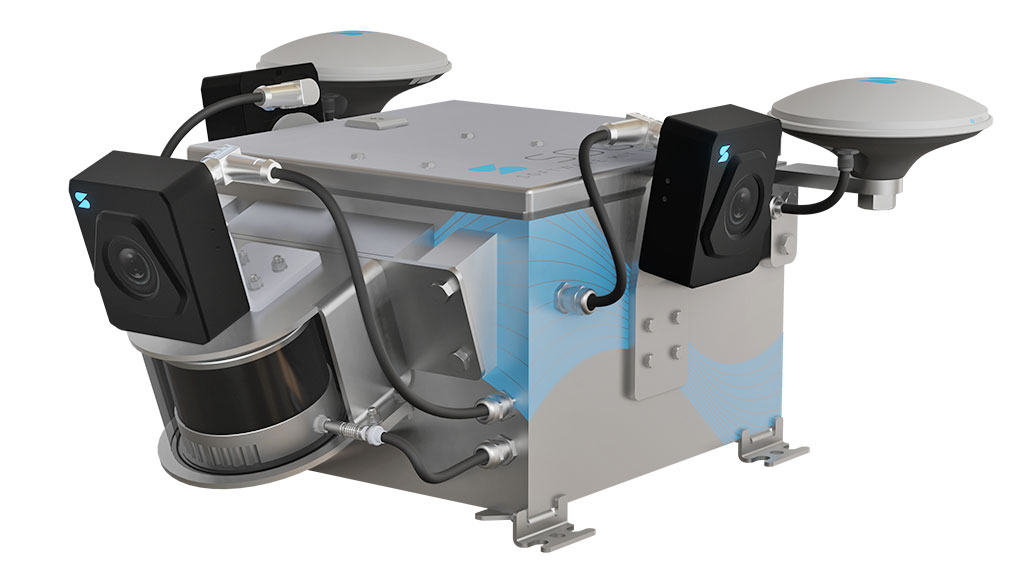
\includegraphics[width=0.6\linewidth]{images/sdx-compact.jpg}
    \caption[SDX-Compact]{The SDX-Compact manufactured by Sodex Innovations GmbH. The set of sensors consists of a 3D LiDAR scanner, three RGB cameras and a high-accuracy positioning system. Image source: \href{https://fieldwork.ch/de/produkte/geopositioning/mobile-datenerfassung/sdx-compact}{Fieldwork}}
    \label{fig:sdx-compact}
\end{figure}

\subsection{LiDAR Sensor}

The SDX-Compact \reffig{sdx-compact} is equipped with a Pandar XT32 \cite{hesai_xt16_32_32m} LiDAR sensor, manufactured by Hesai Technology. This is a mechanical rotating LiDAR with a full $360 \degree$ horizontal field of view and 32 beams distributed vertically, at $1 \degree$ resolution. Horizontal resolution depends on the desired output frequency. With our settings, the sensor produces 10 complete scans per second, resulting in a horizontal resolution of $0.18 \degree$.  The maximum operational range is 120m, but this decreases to 50m for low-reflectivity targets. The official specifications state a typical accuracy of $\pm 1$cm, with precision $\pm 0.5$cm, in a static environment. For each beam, the strongest return is processed, leading to 640,000 points being generated per second. The high output bandwidth is handled by an Ethernet connection, over which points are sent as \acrshort{udp} packets. The sensor also supports \acrshort{ptp} synchronisation, essential for high-quality sensor fusion.

% mention limited fov

\subsection{GNSS/INS receiver}

Another component of the sensor stack is the Septentrio AsteRx SBi3 Pro+ GNSS/INS receiver \cite{Septentrio_AsteRx_SBi3_Pro+}, which provides global positioning and orientation data at a rate of 100Hz. Internally, this relies on two distinct mechanisms.

The localization information comes from a dual antenna GNSS module compatible with several GNSS consellations (e.g. \acrshort{gps}, \acrshort{glonass}, Galileo), to ensure optimal worldwide coverage. In standalone mode, the advertised typical accuracy is 1m, but the receiver also acts as an NTRIP (a protocol for differential GPS) client, gathering correction information, in order to achieve centimeter-level accuracy.

An \acrfull{imu} module records acceleration data and provides the remaining orientation angles (roll, pitch, yaw) to compute the complete pose, in 6 \acrfull{dof}. This is integrated with the absolute GNSS measurements using the patented FUSE+ technology \cite{Septentrio_FUSE_Sensor_Fusion}, resulting in an orientation error below  $\text{5-10}\degree$.

Like any system reliant on satellite communication, this will suffer significantly in situations where the signal propagation is disturbed (heavy clouds, ``urban canyons'', thick vegetation, spoofing), even leading to loss of \emph{\gls{gnssfix}}.

To conclude this section, we recognize and underline the importance of accurate extrinsic calibration between the LiDAR and the local INS coordinate frame, which has to be performed prior to any reliable data collection procedure. Given the radically different modalities of these two sensors, this is not a trivial task \cite{lidar-gps-calib} and is outside the scope of the current work.

\section{Data acquisition}

\section{Solution architecture}







\cleardoublepage

\chapter{Results}
\label{ch:results}

This chapter provides a quantitative and qualitative assessment of our method, by applying it to various scenarios and analysing its output. We begin by formulating a set of odometry and mapping metrics, then observe how our solution behaves if some of its components are altered, and test it on multiple datasets.

\section{Evaluation metrics}
Let us first define the main metrics used for evaluation. In terms of trajectory, Zhang and Scaramuzza \cite{zhang2018tutorial} provide a description of typical metrics for visual odometry, which also apply to LiDAR odometry. Given a ground-truth pose
$\pose_i = \left( \matR_i, \vect_i\right)$ and a corresponding pose
$\widehat{\pose}_i = \left( \widehat{\matR}_i, \widehat{\vect}_i\right)$, we can define translation and rotation errors as:
\begin{equation}
    \begin{aligned}
        e_{\text{trans}}(\vect_i, \widehat{\vect}_i) & = \normtwo{\vect_i- \widehat{\vect}_i} \\
        e_{\text{rot}}(\matR_i, \widehat{\matR}_i )  & = \normtwo{
            \Logmap{\transpose{\widehat{\matR}_i} \matR_i}
        }
        \eqdot
    \end{aligned}
\end{equation}
A simple way to compare two pose sequences that start at the same pose is to compute $e_{\text{trans}}(\vect_N, \widehat{\vect}_N)$ and $e_{\text{rot}}(\matR_N, \widehat{\matR}_N)$, the errors at the final state $N$. A more informative measure is given by the \acrfull{ate} \cite{kummerle2009measuring}:
\begin{equation}
    \begin{aligned}
        \text{ATE}_{\text{trans}} & = \sqrt{\frac{1}{N}\sum_{i=1}^{N} e_{\text{trans}}^2(\vect_i, \widehat{\vect}_i)} \\
        \text{ATE}_{\text{rot}}   & = \sqrt{\frac{1}{N}\sum_{i=1}^{N} e_{\text{rot}}^2(\matR_i, \widehat{\matR}_i )}
        \eqdot
    \end{aligned}
\end{equation}
We compute this after transforming the ground truth and predicted trajectories such that they begin with $\pose_0 = \matx{I}_4$. In the KITTI Benchmark \cite{geiger2012kitti}, this was extended to \acrfull{rte}, a metric that is applied on sub-sequences of a certain length or velocity, for a detailed evaluation. Given a sub-sequence $(i,j)$, we compute
$\vect_{i,j} = \transpose{\matR_i}(\vect_j - \vect_i)$
and
$\matR_{i,j} = \transpose{\matR_i}\matR_j$,
then derive the relative error, as a percentage, using:
\begin{equation}
    \begin{aligned}
        \text{RTE}_{\text{trans}} & =
        \frac{e_{\text{trans}}(\vect_{i,j}, \widehat{\vect}_{i,j})}{\normtwo{\vect_{i,j}}} \cdot 100                  \\
        \text{RTE}_{\text{rot}}   & =\frac{
            e_{\text{rot}}(\matR_{i,j}, \widehat{\matR}_{i,j} ) }{\normtwo{\Logmap{\matR_{i,j}}}} \cdot 100    \eqdot \\
    \end{aligned}
\end{equation}

Addressing one of the research questions that motivated this work, we also aim to quantify the quality of the resulting maps, to observe the improvements we bring to the GNSS-merged point cloud. Surprisingly, existing SLAM solutions rarely include rigorous map evaluation, because the map is seen as a localization-enabling tool, rather than a by-product of the system.
The metrics here are closely related to the registration task, but differ in that they are applied on a complete 3D map, instead of a pair of point sets. We note that computing a single value for an entire point cloud is rather misleading, due to variations that appear between its regions, so we aim for point-based metrics that we can analyse through a histogram and \acrfull{cdf}.

A high-quality 3D map is expected to be dense, consistent, and provide high detail for observed features. A very trivial metric is the nearest-neighbor distance. Without considering degenerate cases, having a small nearest-neighbor distance is desirable, but this is constrained by the resolution of the sensor --- the distance would be small even when point clouds do not align well, if the LiDAR has high resolution.
Alternatively, we can compute the number of points within a given radius from each point. This is a reliable measure of local density, but it is unable to distinguish between randomly-scattered points and a structured region.
Inspired by the point-to-plane distance (Eq.~\ref{eq:p2plane}), we can compute a metric that measures the deviation of each point from the surface determined by its neighborhood. To avoid noise, we evaluate this for regions that have a high chance of representing planar surfaces, indicated by the normal consistency $c$.
If $\vecx{n}$ and \mbox{$\left\{\vecx{n}_1, \dots \vecx{n}_k\right\}$} are the normals of a point and its neighbors, then
\mbox{$c = \modulus{\transpose{\vecx{n}} \frac{1}{k}\sum_{i \in (1, k)} \vecx{n}_i}$}.

\newcommand{\pk}{\vecx{p}_k}
Another useful metric is given by point entropy, as described in \cite{adolfsson2021coral}. Considering all points within a radius $r$ around point $\pk$, we compute the covariance $\matx{\Sigma}(\pk)$, then derive the differential entropy as:
\begin{equation}
    h(\pk) = \frac{1}{2}\text{ln}\left(
    2\pi e \text{det}\left(\matx{\Sigma}(\pk)\right)
    \right)
\end{equation}
Adjusting the neighborhood radius controls the granularity of the metric, with a value around 0.2m providing a fair trade-off between detail level and computational cost.

To assess computational performance, we provide the processing duration (s) indicating the real time taken for a single input scan, without considering pre-processing operations, when executed on an Intel Core i7-10750H CPU.

% Given a set of ground-truth poses
% \mbox{$\mathcal{T} = \left\{ \pose_i \in \SE{3} : \pose_i = \left( \matR_i, \vect_i\right)\right\}$}, and a corresponding set of predicted poses
% \mbox{$
%         \widehat{\mathcal{T}} = \left\{ \widehat{\pose}_i \in \SE{3} : \right\}
%     $}

% define ATE



\section{Parameter analysis}

In this section we discuss some of the main parameters of our method, in order to better understand their effect on performance, trajectory estimation and final map quality.

\subsection{Point cloud voxelization}

\begin{table}[h]

    \centering
    {\small
        \begin{tabular}{c|c|cc|cc|c|cc}
            \hline
            \textbf{Voxel} & \textbf{Median}   & \multicolumn{2}{c|}{ \textbf{ATE}} & \multicolumn{2}{c|}{ \textbf{Final}} & \textbf{Avg.}   & \multicolumn{2}{c}{ \textbf{Avg. Corr.}}                                                       \\
            \textbf{Size}  & \textbf{Duration} & \textbf{tra.}                      & \textbf{rot.}                        & \textbf{tra.}   & \textbf{rot.}                            & \textbf{RMSE}   & \textbf{tra.}   & \textbf{rot.}   \\
            (m)            & (s)               & (m)                                & (rad)                                & (m)             & (rad)                                    & (m)             & (m)             & (rad)           \\
            \hline
            \hline
            0.1            & 0.2984            & \textbf{1.2814}                    & \textbf{0.0294}                      & \textbf{2.5337} & \textbf{0.0467}                          & \textbf{0.0555} & \textbf{0.0080} & \textbf{0.0010} \\
            0.2            & 0.1684            & 1.3858                             & 0.0315                               & 2.7607          & 0.0511                                   & 0.0868          & 0.0210          & 0.0024          \\
            0.3            & \textbf{0.1586}   & 1.5499                             & 0.0347                               & 3.0500          & 0.0542                                   & 0.1206          & 0.0351          & 0.0040          \\
            0.4            & 0.1589            & 1.7736                             & 0.0418                               & 3.5078          & 0.0659                                   & 0.1545          & 0.0519          & 0.0055          \\
            0.5            & 0.1603            & 1.4667                             & 0.0358                               & 2.9164          & 0.0568                                   & 0.1876          & 0.0819          & 0.0077          \\
            0.6            & 0.1635            & 1.9237                             & 0.0475                               & 3.7190          & 0.0677                                   & 0.2186          & 0.1069          & 0.0116          \\
            \hline
        \end{tabular}
    }
    \caption{Metrics for varying voxel sizes, on a sequence of 500 LiDAR scans. \\Using a very small voxel size (< 0.1m) increases computational cost and does not help with reducing point cloud noise, so we do not include that. We also report average RMSE values (after registration), alongside the average correction computed by GICP after the ICP alignment. The duration does not directly depend on the voxel size, because more ICP iterations are required for registration, when a larger voxel size is used. Overall, a smaller voxel size results in better odometry estimation and higher-quality mapping.}
    \label{tab:voxel_metrics}
\end{table}


Following the motion compensation applied during dataset pre-processing, every input point cloud undergoes a voxelization step (as described in Section~\ref{subsec:registration}) designed to reduce sensor noise while keeping a sufficient amount of information for registration. We select a subsection of the trajectory consisting of 500 LiDAR scans captured over approx.~114m at 8km/h, and execute the pipeline in LiDAR-only mode (disregarding the GNSS information), with multiple voxel size values. As there are no GPS constraints, the graph optimization step does not modify the pose priors computed by LiDAR odometry. The corresponding GPS trajectory is treated as ground-truth, due to its low uncertainty. The results of this evaluation are presented in Table~\ref{tab:voxel_metrics}. Using a larger voxel size decreases the computational cost, as the point clouds involved have smaller resolution, but introduces considerable problems for odometry estimation, as indicated by the ATE values. We also look at the resulting maps, to confirm that a small voxel size leads to higher-quality mapping, as shown in \reffig{voxel-size-mapping}.

\begin{figure}[h]
    \centering
    \subcaptionbox{Distribution of point entropies.}{
        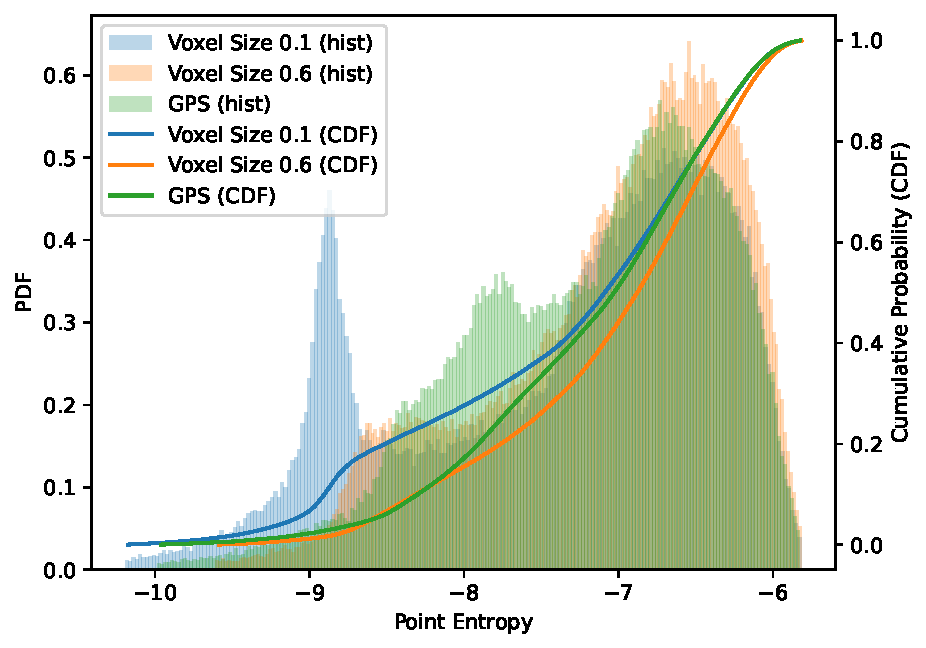
\includegraphics[width=0.45\linewidth]{images/voxel-size-entropy.pdf}
    }
    \hspace{1pt}
    \subcaptionbox{Visual comparison. }{
        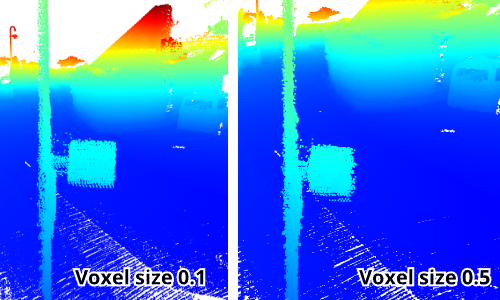
\includegraphics[width=0.45\linewidth]{images/voxel-size-comp.png}
    }
    \caption[Voxel size effect on map quality]{Voxel size effect on map quality: a smaller voxel size results in more accurate registration, leading to lower entropy and sharper edges.}
    \label{fig:voxel-size-mapping}
\end{figure}



% \begin{figure}[h]
%     \centering
%     \subcaptionbox{Translation corrections.}{
%         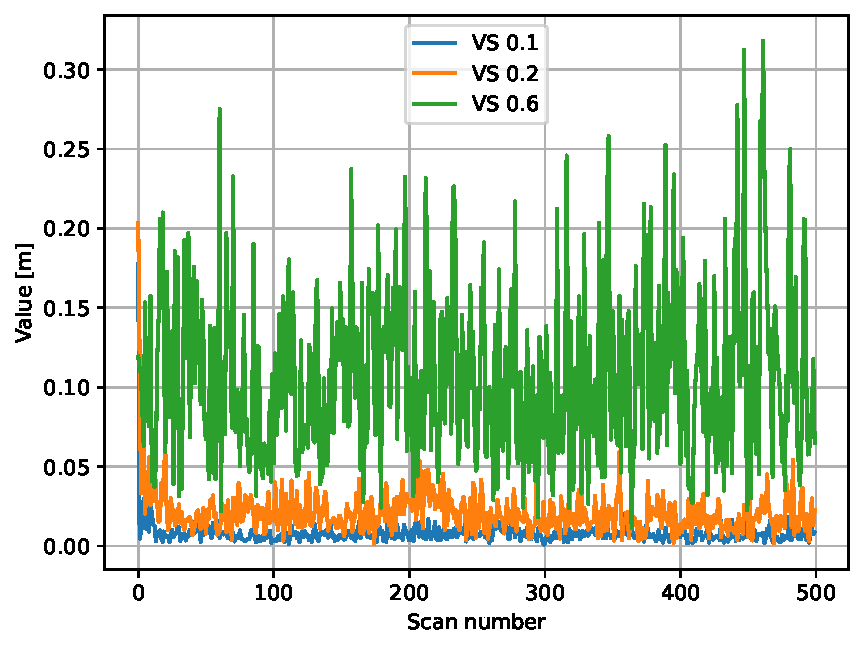
\includegraphics[width=0.46\linewidth]{images/gicp_corrections_trans.pdf}
%     }
%     \hspace{1pt}
%     \subcaptionbox{Rotation corrections.}{
%         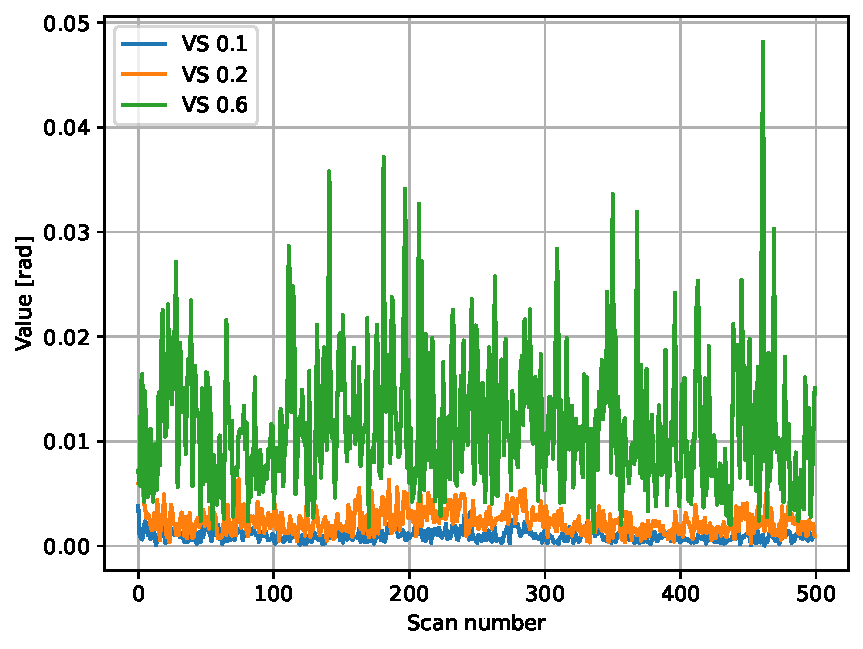
\includegraphics[width=0.45\linewidth]{images/gicp_corrections_rot.pdf}
%     }
%     \caption[]{
%     }
%     \label{fig:gicp-corrections}
% \end{figure}

\subsection{Local map size}
%% how do the results change, depending on the number of previous scans stored

\begin{table}[h]
    \centering
    {\small
        \begin{tabular}{c|c|cc|cc|c|cc}
            \hline
            \textbf{Map}  & \textbf{Median}   & \multicolumn{2}{c|}{ \textbf{ATE}} & \multicolumn{2}{c|}{ \textbf{Final}} & \textbf{Avg.}   & \multicolumn{2}{c}{ \textbf{Avg. Corr.}}                                                       \\
            \textbf{Size} & \textbf{Duration} & \textbf{tra.}                      & \textbf{rot.}                        & \textbf{tra.}   & \textbf{rot.}                            & \textbf{RMSE}   & \textbf{tra.}   & \textbf{rot.}   \\
            (scans)       & (s)               & (m)                                & (rad)                                & (m)             & (rad)                                    & (m)             & (m)             & (rad)           \\
            \hline
            \hline

            1             & 0.2349            & 5.0058                             & 0.1564                               & 10.2891         & 0.2603                                   & 0.0940          & 0.0366          & 0.0021          \\
            2             & \textbf{0.2308}   & 4.3812                             & 0.1355                               & 9.1949          & 0.2318                                   & 0.0818          & 0.0171          & 0.0016          \\
            5             & 0.2632            & 1.8325                             & 0.0458                               & 3.6849          & 0.0734                                   & 0.0615          & 0.0094          & 0.0011          \\
            10            & 0.2962            & 1.2814                             & 0.0294                               & 2.5337          & 0.0467                                   & 0.0555          & 0.0080          & \textbf{0.0010} \\
            15            & 0.3242            & 1.1645                             & 0.0263                               & 2.2848          & 0.0415                                   & 0.0540          & \textbf{0.0076} & \textbf{0.0010} \\
            25            & 0.3984            & \textbf{1.1040}                    & \textbf{0.0245}                      & \textbf{2.1504} & \textbf{0.0384}                          & \textbf{0.0531} & 0.0079          & 0.0011          \\
            \hline
        \end{tabular}
    }
    \caption{Metrics for varying map sizes, on a sequence of 500 LiDAR scans. As more past scans are used to build the local map, the registration step becomes slower, but the odometry error decreases. We use 10 previous scans, as that provides a good balance between speed and accuracy.}
    \label{tab:map_sizes}
\end{table}

In this experiment, we observe the behavior of the algorithm in relation to the size of the local map, \ie the number of previous scans that the registration is performed against. Given the high frequency and operational range of the sensor, consecutive scans have large overlapping areas which represent useful cues for point cloud alignment. This is proven by the low odometry errors obtained for map size $\geq 5$ in Table~\ref{tab:map_sizes}. When larger maps are used, the computational time increases, without significant improvements for trajectory estimation.



\begin{table}[h]
    \centering
    {\small
        \begin{tabular}{c|c|cc|cc|c|cc}
            \hline
            \textbf{GICP}    & \textbf{Median}   & \multicolumn{2}{c|}{ \textbf{ATE}} & \multicolumn{2}{c|}{ \textbf{Final}} & \textbf{Avg.}   & \multicolumn{2}{c}{ \textbf{Avg. Corr.}}                                                       \\
            \textbf{thresh.} & \textbf{Duration} & \textbf{tra.}                      & \textbf{rot.}                        & \textbf{tra.}   & \textbf{rot.}                            & \textbf{RMSE}   & \textbf{tra.}   & \textbf{rot.}   \\
            (m)              & (s)               & (m)                                & (rad)                                & (m)             & (rad)                                    & (m)             & (m)             & (rad)           \\
            \hline
            \hline
            -                & \textbf{0.2111}   & 1.8036                             & 0.0371                               & 2.8009          & 0.0571                                   & 0.0601          & -               & -               \\
            0.1              & 0.2949            & 1.1686                             & \textbf{0.0275}                      & 1.5486          & 0.0357                                   & \textbf{0.0457} & \textbf{0.0070} & \textbf{0.0009} \\
            0.2              & 0.3020            & \textbf{1.1167}                    & 0.0280                               & \textbf{1.4442} & \textbf{0.0340}                          & 0.0520          & \textbf{0.0070} & \textbf{0.0009} \\
            0.5              & 0.2860            & 1.1958                             & 0.0326                               & 1.4858          & 0.0390                                   & 0.0599          & 0.0073          & 0.0010          \\
            \hline
        \end{tabular}
    }
    \caption{Metrics for GICP variations, on a sequence of 500 LiDAR scans. We use GICP in order to improve surface alignment, as a second registration step after robust ICP. Having a larger correspondence threshold increases the risk of selecting incorrect point pairs, but helps align sparse regions of the scans.}
    \label{tab:gicp_variations}
\end{table}
\begin{figure}[H]
    \centering
    \subcaptionbox{Trajectory end point location. \label{fig:gicp-result-xy}}{
        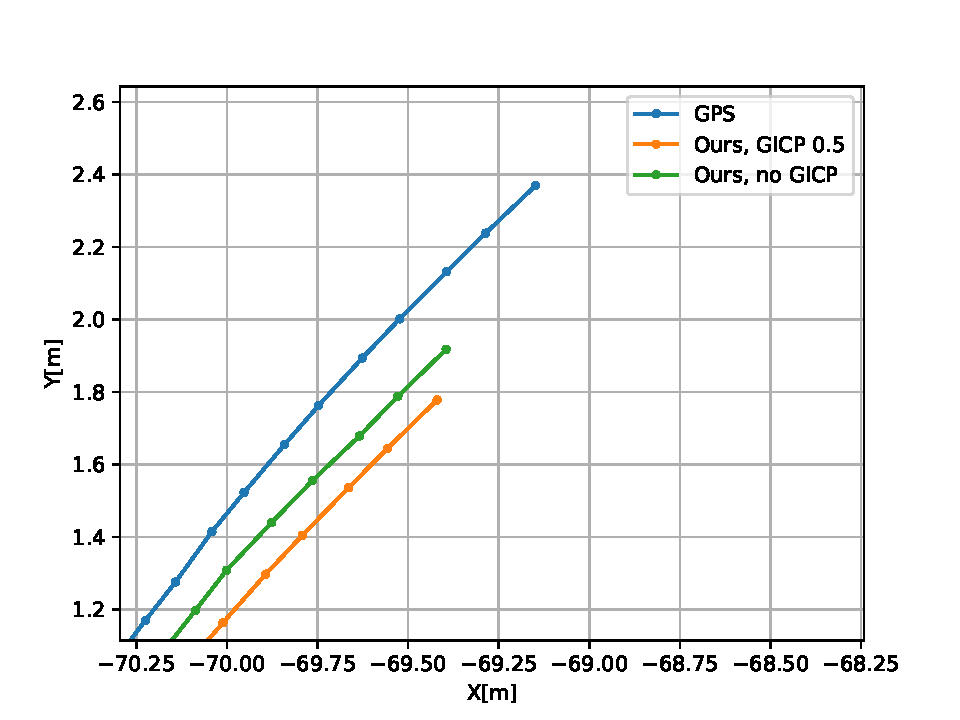
\includegraphics[width=0.47\linewidth]{images/gicp-result-xy.pdf}
    }
    \hspace{1pt}
    \subcaptionbox{Z error evolution.\label{fig:gicp-z-error}}{
        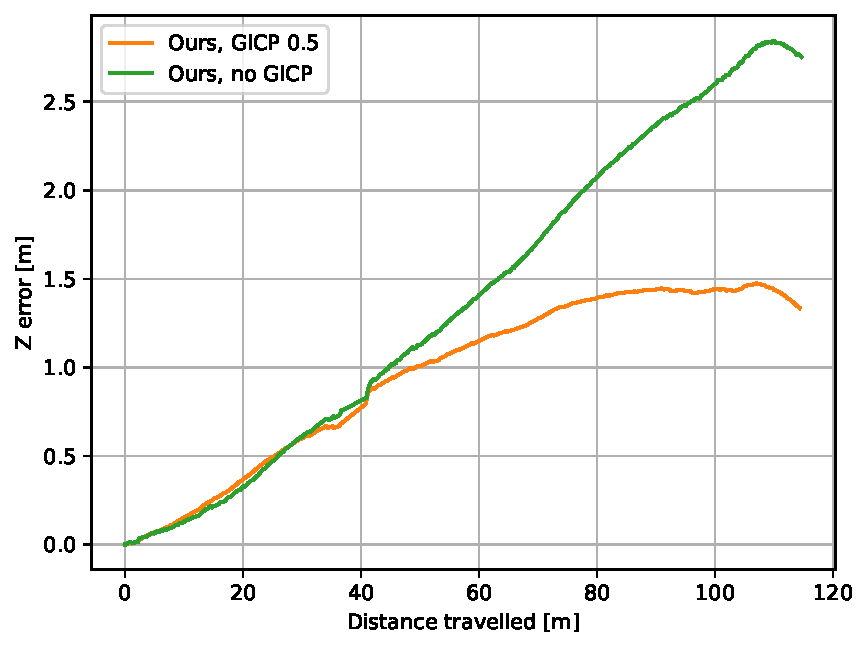
\includegraphics[width=0.44\linewidth]{images/gicp-z-error.pdf}
    }
    \caption[Trajectory evaluation with and without GICP]{Trajectory evaluation with and without GICP. The additional GICP registration step reduces the Z-alignment error.}
    \label{fig:gicp-traj-result}
\end{figure}

\subsection{Registration strategy}
%% how do the results change, depending on whether we use GICP or not

We also assess the influence of the Generalized ICP registration step. During the experimental phase, we observed that this has a very positive effect on accurately matching the ground plane, and this is confirmed by the metrics in Table~\ref{tab:gicp_variations}. For a more thorough analysis, we show the results corresponding to several distance threshold values, and compare against the case where only point-to-point ICP is used. The no-GICP version leads to higher trajectory errors overall, but we note that the Z component (elevation) has the highest contribution to this error. The XY error is smaller when GICP is not used~\reffigbr{gicp-result-xy}, but the Z error is almost doubled \reffigbr{gicp-z-error}. In terms of map quality, using GICP clearly helps reduce point entropies and point-to-plane errors, so the surfaces of the output map capture more details, but additional constraints (\ie GPS) will help prevent drifts.

\begin{figure}[H]
    \centering
    \subcaptionbox{Distribution of point entropies.}{
        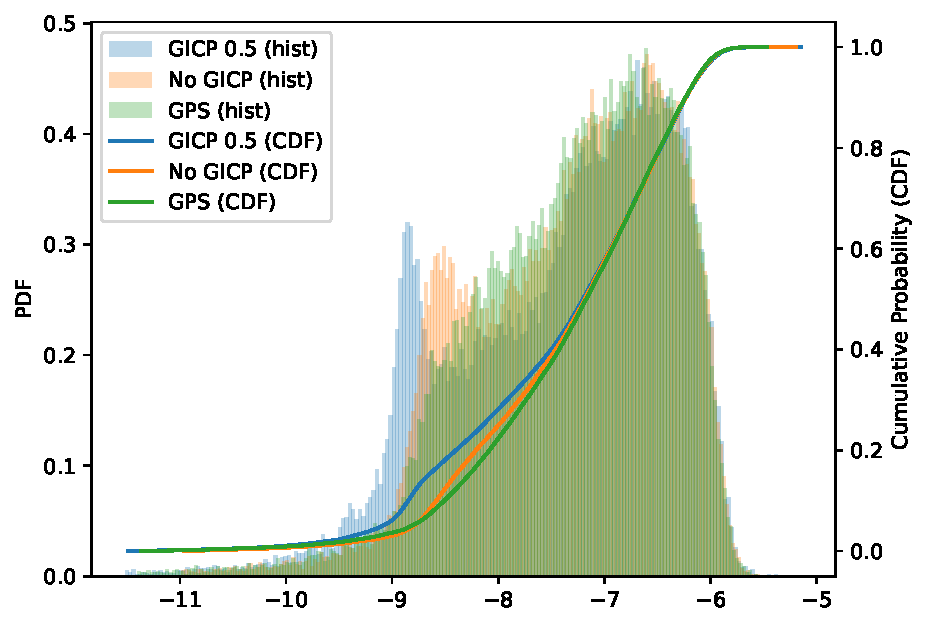
\includegraphics[width=0.46\linewidth]{images/gicp-map-entropy.pdf}
    }
    \hspace{1pt}
    \subcaptionbox{Point-to-plane errors (first 30 scans)}{
        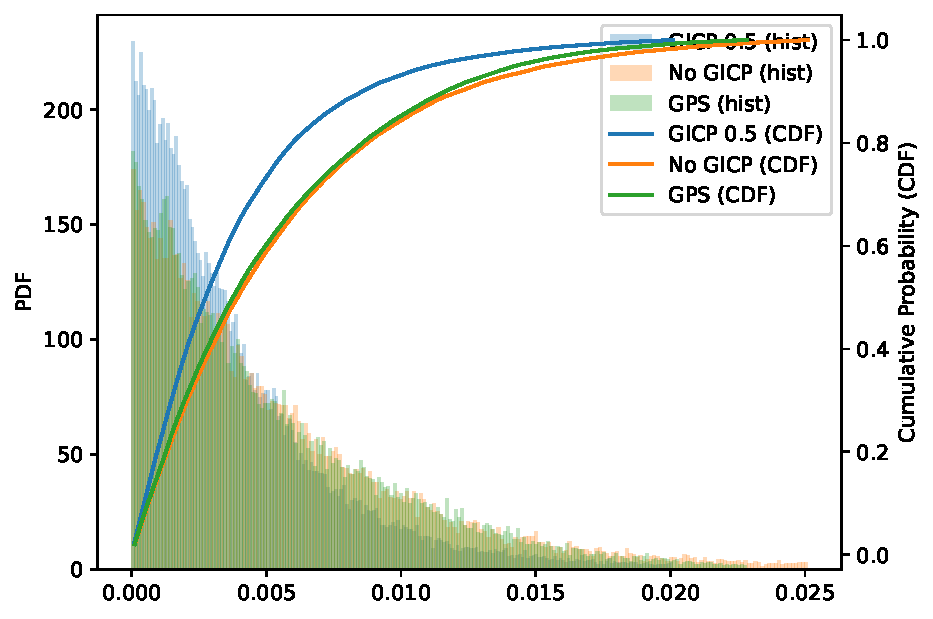
\includegraphics[width=0.45\linewidth]{images/gicp-p2plane.pdf}
    }
    % \subcaptionbox{Observing the Z difference in CloudCompare. Yellow - without GICP, white - with GICP.}{
    %     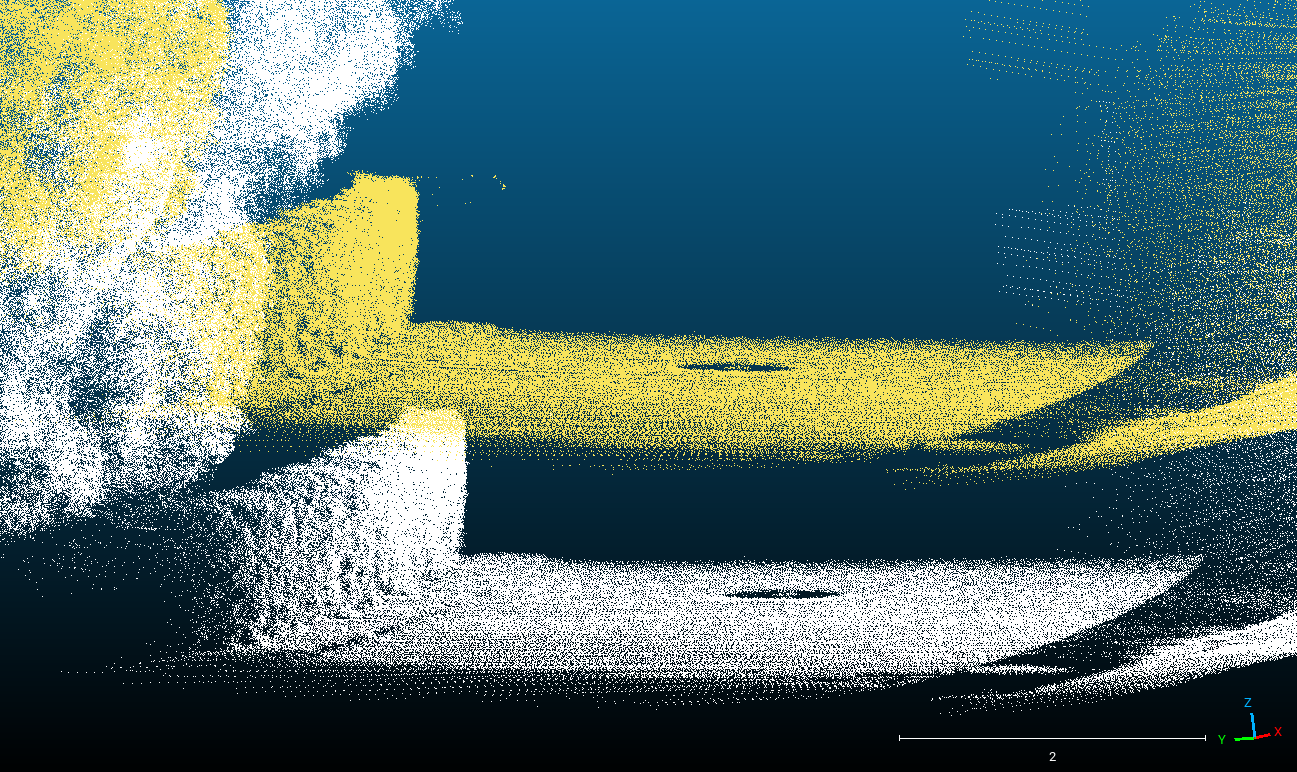
\includegraphics[width=0.45\linewidth]{images/gicp-z-error-view.png}
    % }
    \caption[Map evaluation with and without GICP]{Map evaluation with and without GICP. Entropy and point-to-plane errors are lower, when GICP is used, indicating a higher-quality map.}
    \label{fig:gicp-map-result}
\end{figure}


\section{Odometry evaluation}

The first odometry evaluation we perform is on the trajectory recorded with the \mbox{SDX-Compact} system, depicted in \reffig{odom-traj}. We do not use the GPS data during execution, but treat it as ground truth to obtain the trajectory error metrics in Table~\ref{tab:custom-traj-results}. Because we consider scan timestamps during motion prediction, we are able to handle large ``jumps'' in the scan sequence \reffigbr{odom-jumps}, something that other methods struggle with. However, elevation estimation is still an issue, as seen in \reffig{z-dif-traj}.

\begin{figure}[h]
    \centering
    \subcaptionbox{Full trajectory comparison.}{
        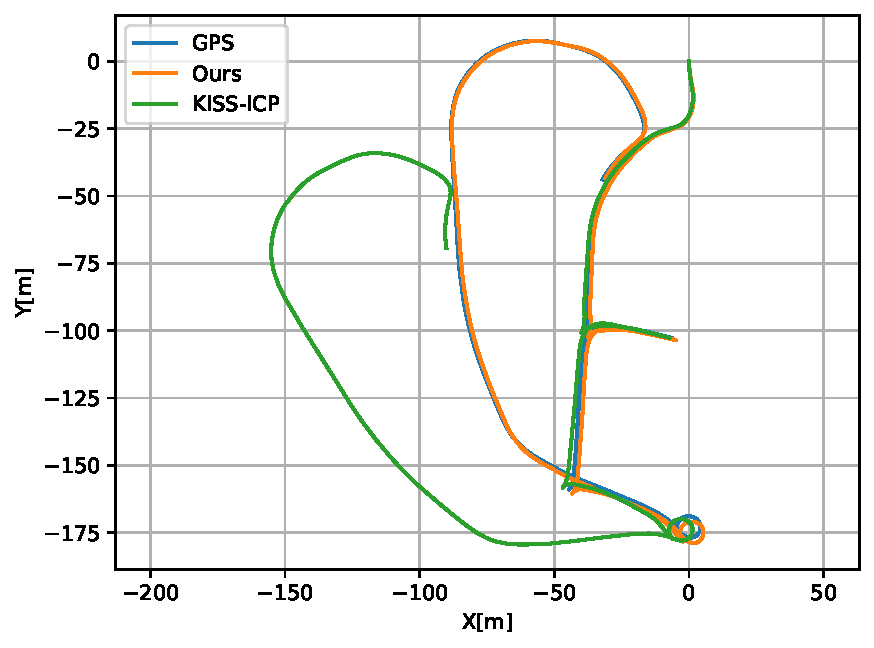
\includegraphics[width=0.445\linewidth]{images/eval_traj/traj.pdf}
    }
    \hspace{1pt}
    \subcaptionbox{A troublesome region with time jumps. \label{fig:odom-jumps}}{
        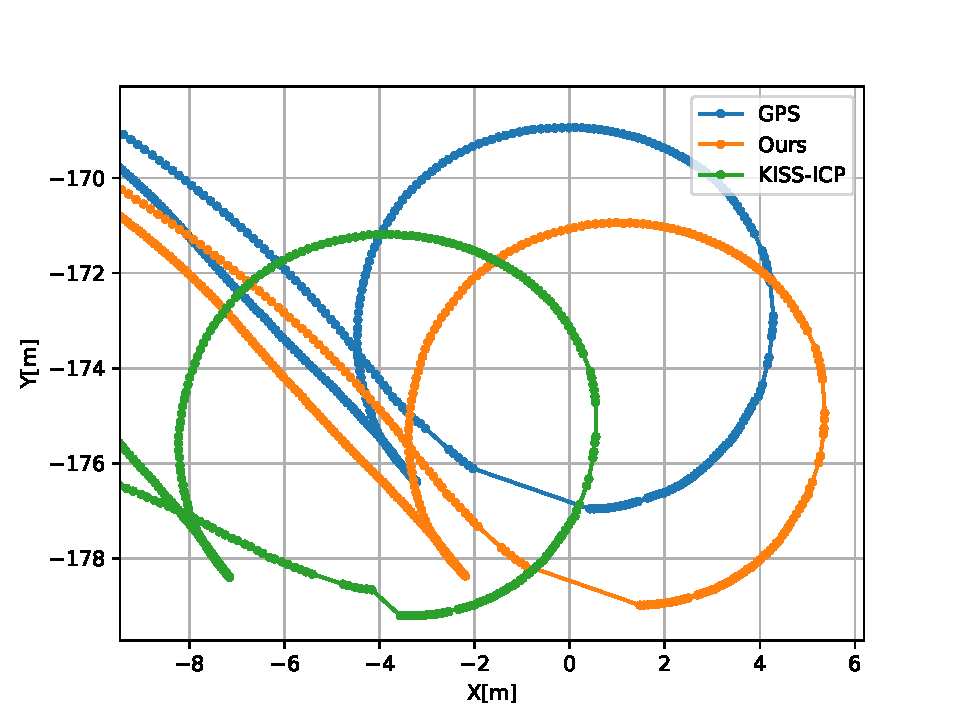
\includegraphics[width=0.485\linewidth]{images/eval_traj/loop.pdf}
    }
    \caption[Odometry evaluation on custom trajectory]{Odometry evaluation on custom trajectory: our method and KISS-ICP \cite{vizzo2023ral} against GPS data.}
    \label{fig:odom-traj}
\end{figure}

\begin{table}[h]
    \centering
    {\small
        \begin{tabular}{c|ccc|ccc|ccc}
            \hline
                     & \multicolumn{3}{c|}{\textbf{ATE}} & \multicolumn{3}{c|}{\textbf{Final}} & \multicolumn{3}{c}{\textbf{Avg. RTE} (100m)}                                                                                                  \\
                     & \textbf{XY}                       & \textbf{tra.}                       & \textbf{rot.}                                & \textbf{XY}   & \textbf{tra.} & \textbf{rot.} & \textbf{XY}   & \textbf{tra.} & \textbf{rot.}  \\
                     & (m)                               & (m)                                 & (rad)                                        & (m)           & (m)           & (rad)         & (\%)          & (\%)          & (\%)           \\
            \hline
            \multicolumn{10}{c}{Full trajectory (644.4m)}                                                                                                                                                                                      \\
            \hline
            KISS-ICP & 34.68                             & 35.21                               & 0.32                                         & 50.82         & 51.65         & 0.58          & 31.32         & 36.21         & 111.87         \\
            Ours     & \textbf{1.68}                     & \textbf{8.23}                       & \textbf{0.1}                                 & \textbf{1.08} & \textbf{1.31} & \textbf{0.1}  & \textbf{1.23} & \textbf{2.49} & \textbf{16.26} \\
            \hline
            \multicolumn{10}{c}{Initial section of trajectory (216m)}                                                                                                                                                                          \\
            \hline
            KISS-ICP & \textbf{0.77}                     & \textbf{4.04}                       & 0.08                                         & \textbf{1.33} & \textbf{4.55} & 0.10          & \textbf{0.29} & 4.97          & 38.37          \\
            Ours     & 1.33                              & 5.07                                & 0.08                                         & 2.11          & 8.95          & 0.10          & 0.63          & \textbf{2.64} & \textbf{24.35} \\
            \hline
        \end{tabular}
    }
    \caption{Comparison with KISS-ICP \cite{vizzo2023ral} on custom trajectory. We report average RTE for sub-sequences 100m. KISS-ICP performs better when the scans are captured at equal intervals, but diverges as soon as a significant jump occurs.}
    \label{tab:custom-traj-results}
\end{table}

\begin{figure}[h]
    \centering
    \subcaptionbox{XY errors. The KISS-ICP method diverges after a jump in the sequence.}{
        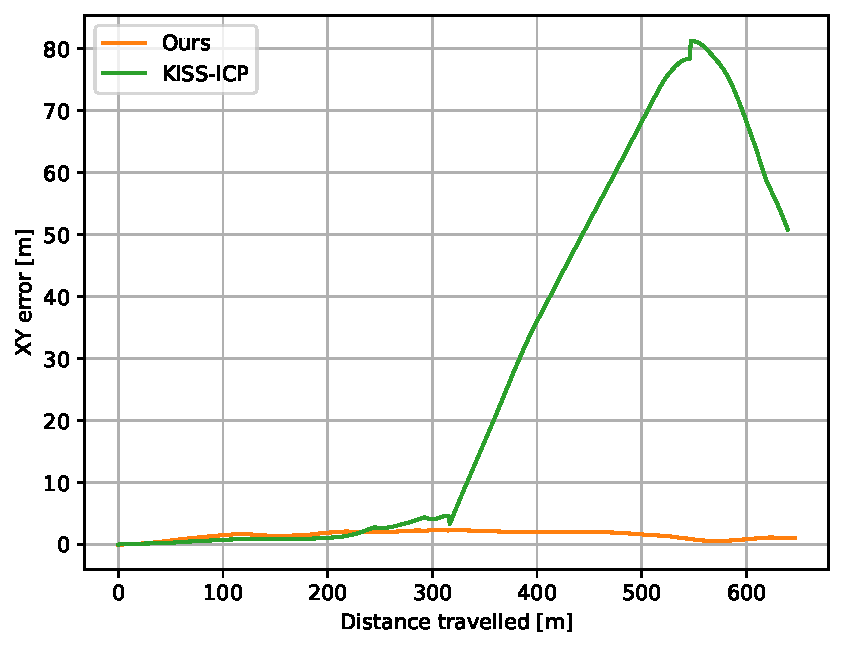
\includegraphics[width=0.455\linewidth]{images/eval_traj/xy_errors.pdf}
    }
    \hspace{1pt}
    \subcaptionbox{Z values. Both methods struggle to correctly estimate the Z component of the location. \label{fig:z-dif-traj}}{
        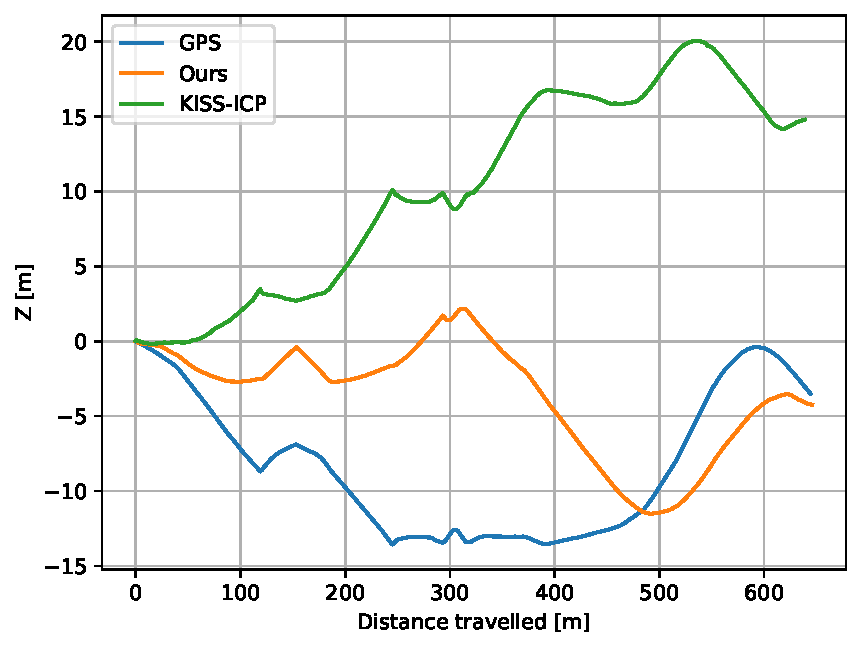
\includegraphics[width=0.475\linewidth]{images/eval_traj/Zs.pdf}
    }
    \caption[Position analysis on custom trajectory]{Position analysis on custom trajectory. }
    \label{fig:xyz-traj}
\end{figure}

We also evaluate on the sequences of the KITTI dataset \cite{geiger2013vision} which include ground-truth pose values from a GPS + IMU sensor system. This is a popular benchmark for urban SLAM problems, and it represents an interesting challenge for our solution because it uses a different LiDAR sensor (Velodyne HDL-64E), the environment is different, and moving vehicles are present. To operate on this dataset, we adjust the solution as follows:
\begin{compactitem}
    \item Discard LiDAR points that are farther than 50m or closer than 1m, to avoid high distortion and points belonging to the sensor rig
    \item Use a larger base voxel size: as the scanned environment is larger, we use a default voxel size of 0.2m instead of 0.1m
\end{compactitem}
The results of this evaluation are presented in Table~\ref{tab:odom-kitti} and Figure~\ref{fig:kitti-traj}.

\begin{table}[h]
    \centering
    {\small
        \begin{tabular}{c|c|ccc|ccc|ccc}
            \hline
                          &                 & \multicolumn{3}{c|}{\textbf{ATE}} & \multicolumn{3}{c|}{\textbf{Final}} & \multicolumn{3}{c}{\textbf{Avg. RTE} (100m)}                                                                                                \\
            \textbf{Seq.} & \textbf{Length} & \textbf{XY}                       & \textbf{tra.}                       & \textbf{rot.}                                & \textbf{XY}   & \textbf{tra.} & \textbf{rot.} & \textbf{XY}  & \textbf{tra.} & \textbf{rot.} \\
                          & (m)             & (m)                               & (m)                                 & (rad)                                        & (m)           & (m)           & (rad)         & (\%)         & (\%)          & (\%)          \\
            \hline \hline
            00            & 3723.24         & 7.29                              & 16.28                               & 0.07                                         & 10.59         & 11.58         & 0.06          & 0.81         & 1.23          & 12.88         \\
            01            & 2453.26         & 24.53                             & 190.1                               & 0.21                                         & 39.9          & 291.51        & 0.3           & 0.98         & 1.31          & 45.7          \\
            02            & 5067.02         & 22.2                              & 50.39                               & 0.13                                         & 49.72         & 99.53         & 0.22          & 0.7          & 1.22          & 11.99         \\
            03            & 560.85          & 2.92                              & 8.84                                & 0.05                                         & 6.35          & 18.15         & 0.08          & 0.57         & \textbf{0.67} & 7.69          \\
            04            & 393.65          & 0.72                              & 4.98                                & 0.03                                         & 1.16          & 11.76         & 0.06          & 0.39         & 0.89          & 125.81        \\
            05            & 2205.2          & 4.62                              & 6.92                                & 0.04                                         & 9.2           & 13.79         & 0.07          & \textbf{0.5} & 1.02          & 20.44         \\
            06            & 1232.69         & 2.03                              & 3.78                                & 0.03                                         & 4.88          & 8.79          & 0.05          & 0.59         & 0.91          & 54.07         \\
            07            & 694.39          & \textbf{0.5}                      & \textbf{1.8}                        & \textbf{0.02}                                & \textbf{0.96} & \textbf{1.36} & \textbf{0.02} & 0.58         & 1.0           & \textbf{5.12} \\
            08            & 3222.02         & 16.73                             & 28.33                               & 0.08                                         & 20.9          & 33.15         & 0.11          & 1.04         & 1.52          & 24.66         \\
            09            & 1704.96         & 6.12                              & 14.12                               & 0.06                                         & 9.28          & 9.78          & 0.04          & 0.68         & 1.03          & 8.1           \\
            10            & 919.4           & 3.94                              & 18.8                                & 0.07                                         & 4.61          & 21.78         & 0.09          & 0.65         & 1.04          & 8.79          \\
            \hline
        \end{tabular}
    }
    \caption{Odometry evaluation on KITTI sequences. We report the XY-only error values to emphasize localization performance. RTE values are averaged over all 100m sub-sequences. Like most dead-reckoning solutions, the ATE and Final errors increase with the length of the trajectory.}
    \label{tab:odom-kitti}
\end{table}

\begin{figure}[h]
    \centering
    \subcaptionbox{Sequence 00.}{
        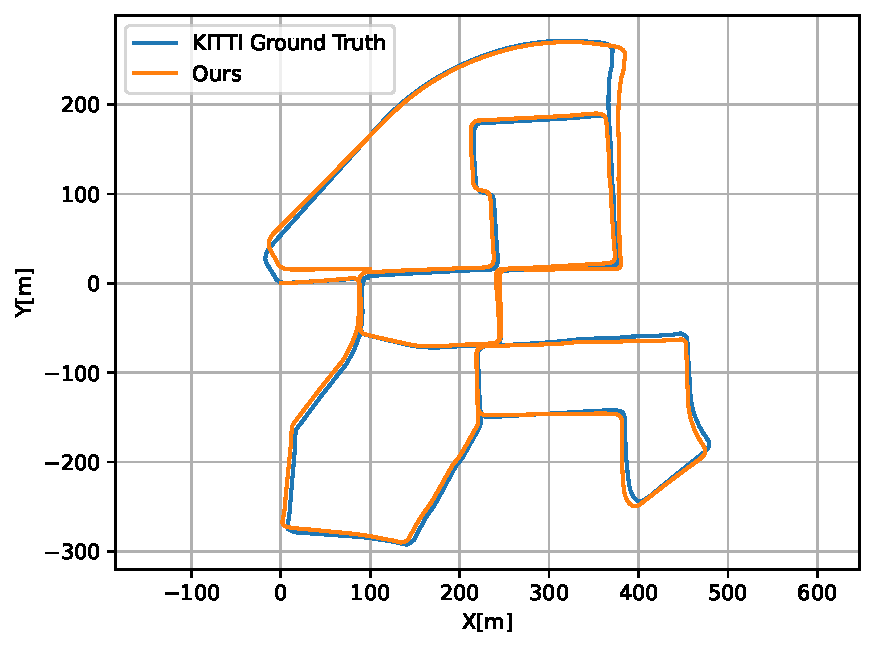
\includegraphics[width=0.3\linewidth]{images/kitti/00.pdf}
    }
    \subcaptionbox{Sequence 02.}{
        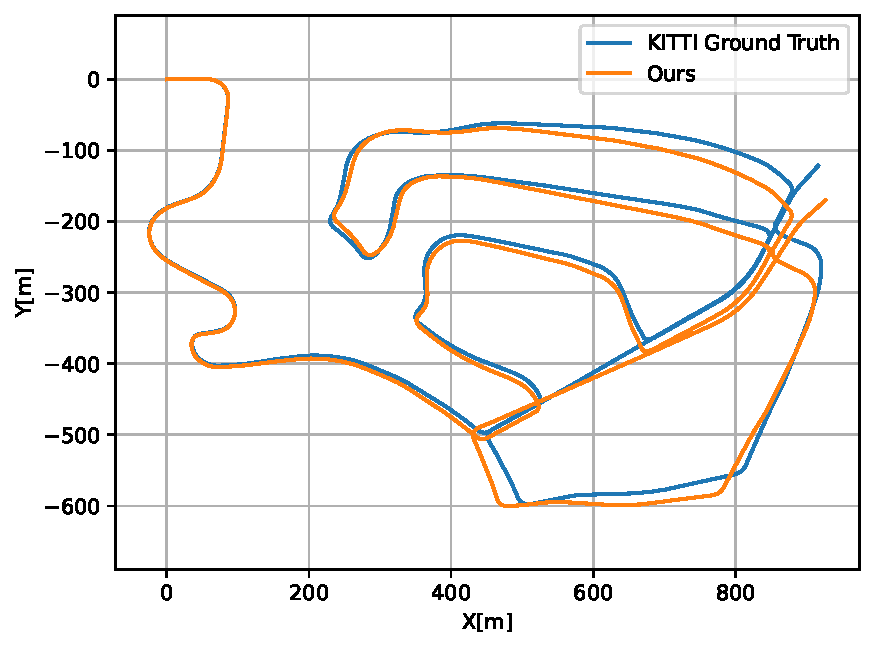
\includegraphics[width=0.3\linewidth]{images/kitti/02.pdf}
    }
    \subcaptionbox{Sequence 08.}{
        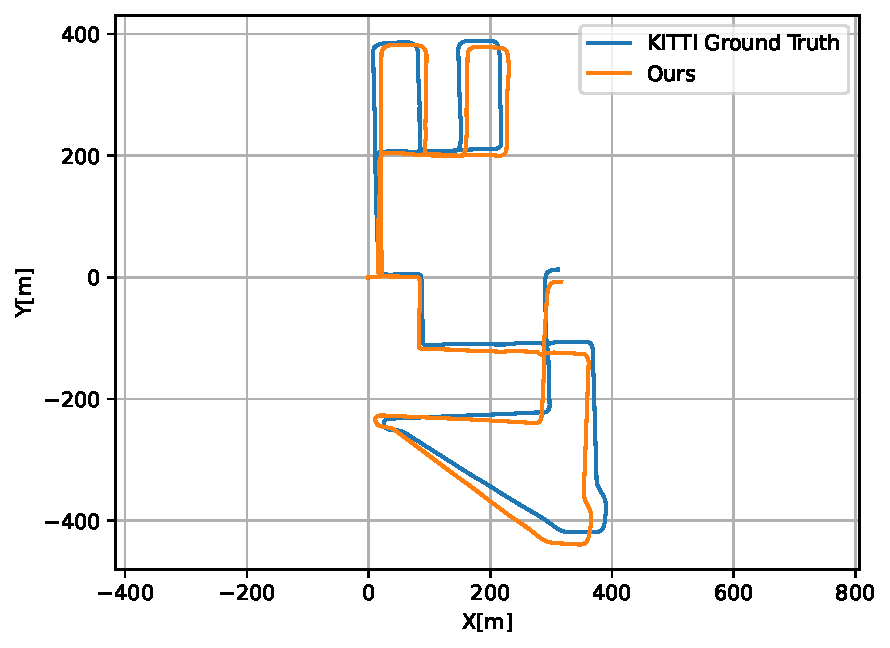
\includegraphics[width=0.3\linewidth]{images/kitti/08.pdf}
    }
    \caption[Odometry evaluation on KITTI sequences]{Odometry results on the three longest KITTI sequences.}
    \label{fig:kitti-traj}
\end{figure}

\section{GPS-integrated evaluation}
% using noisy gps on our data

So far, our method has been evaluated without any GPS input, essentially acting as a LiDAR-based dead-reckoning solution. In this section, we use the data from the GNSS receiver to imitate a real use-case, and assess the trajectory against a GPS-only approach.

First, we would like to observe how robust the solution is to GPS noise, to mimic a scenario where RTK data is not available, or the GPS signal is very poor. Starting from the existing GPS readings, we introduce artificial noise to the location values by sampling a zero-mean Gaussian distribution for each component, and modify the associated covariance based on the $\sigma$ of the noise distribution. The resulting readings and covariance values are used as input for the method, simulating signal scatter. IMU readings are not affected, but we increase the covariance of the orientation components by 0.01, to allow for adjustments from the graph optimization component. We present the results of this experiment in Table~\ref{tab:gps-noisy}, by comparing the noisy GPS input and the output of our method against the accurate GPS location readings. The same phenomenon is shown in Figure~\ref{fig:gps-noise-correction}.

% 0cm, 5cm, 10cm, 50cm, 100cm, 500cm
% Table columns:
% Noise sigma, 

\begin{table}[h!]
    \centering
    {\small
        \begin{tabular}{c|ccccc|ccccc}
            \hline
            \textbf{Noise} $\sigma$ & \multicolumn{5}{c|}{\textbf{Noisy GPS Input}} & \multicolumn{5}{c}{\textbf{Ours}}                                                                                                                                                                                                     \\
            (m)                     & \multicolumn{2}{c}{\textbf{ATE} (m)}          & \multicolumn{3}{c|}{\textbf{Roughness} (m)} & \multicolumn{2}{c}{\textbf{ATE} (m)} & \multicolumn{3}{c}{\textbf{Roughness} (m)}                                                                                                       \\
                                    & \textbf{XY}                                   & \textbf{tra.}                               & \textbf{X}                           & \textbf{Y}                                 & \textbf{Z}     & \textbf{XY}    & \textbf{tra.}  & \textbf{X}     & \textbf{Y}     & \textbf{Z}     \\
            \hline
            \hline
            0.05                    & \textbf{0.114}                                & \textbf{0.134}                              & \textbf{0.005}                       & \textbf{0.007}                             & \textbf{0.002} & \textbf{0.029} & \textbf{0.032} & \textbf{0.003} & \textbf{0.005} & \textbf{0.000} \\
            0.1                     & 0.228                                         & 0.268                                       & 0.011                                & 0.014                                      & 0.009          & 0.058          & 0.067          & \textbf{0.003} & \textbf{0.005} & 0.001          \\
            0.5                     & 1.140                                         & 1.340                                       & 0.218                                & 0.241                                      & 0.228          & 0.285          & 0.571          & 0.015          & 0.018          & 0.013          \\
            1.0                     & 2.280                                         & 2.680                                       & 0.866                                & 0.947                                      & 0.910          & 0.707          & 1.219          & 0.058          & 0.064          & 0.056          \\
            2.0                     & 4.559                                         & 5.359                                       & 3.457                                & 3.768                                      & 3.641          & 2.165          & 7.623          & 0.2            & 0.212          & 0.223          \\
            \hline
        \end{tabular}
    }
    \caption[Trajectory evaluation with noisy GPS]{Trajectory evaluation with noisy GPS input, on a sequence of 1000 LiDAR scans~(approx. 131.7m), against the zero-noise GPS readings. Roughness is measured by fitting a cubic polynomial to subsequences of each dimension --- X, Y and Z, as a function of time --- and averaging the fitting error across all subsequences. Our method is able to filter out GPS noise, reconstructing a trajectory that is smoother and closer to the ground truth.}
    \label{tab:gps-noisy}
\end{table}
\begin{figure}[h]
    \centering
    \subcaptionbox{A straight region.}{
        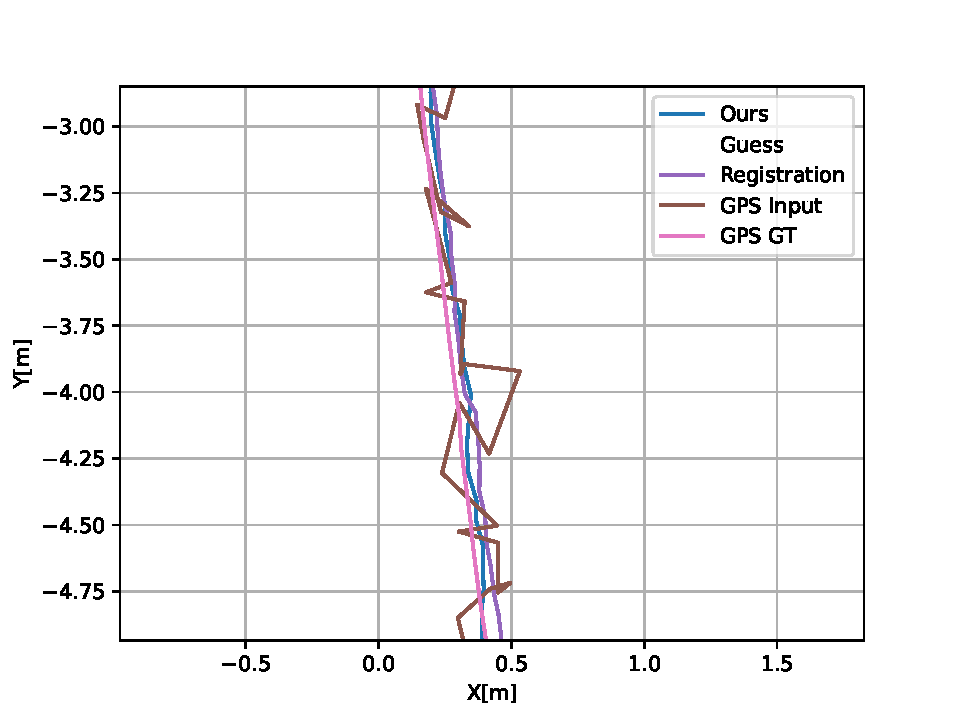
\includegraphics[width=0.475\linewidth]{images/noisy_gps/noisy_01.pdf}
    }
    \subcaptionbox{A corner region.}{
        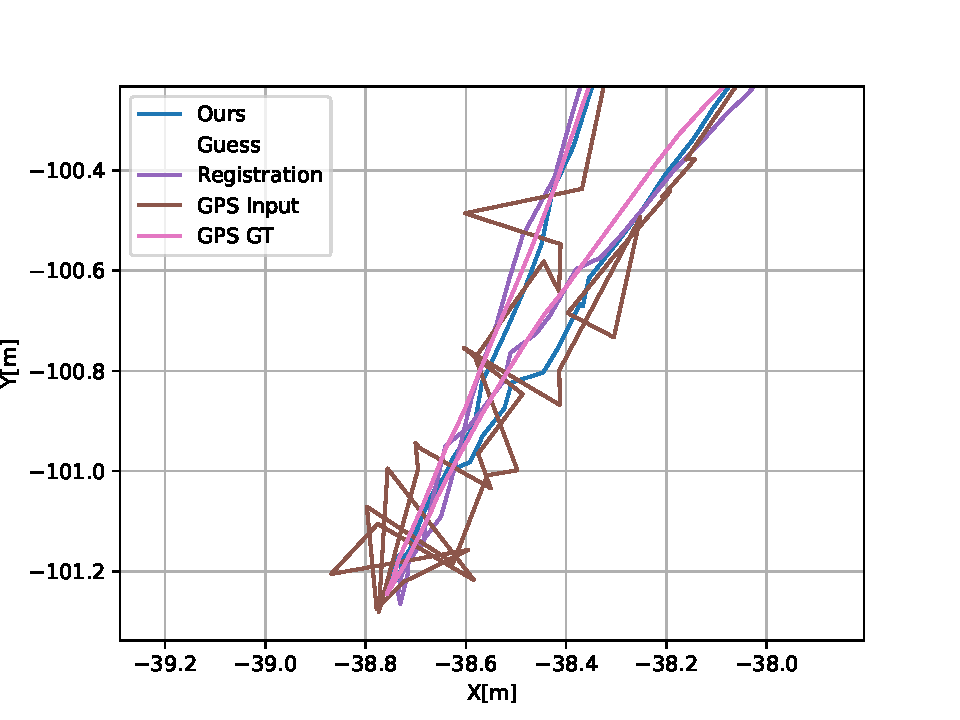
\includegraphics[width=0.475\linewidth]{images/noisy_gps/noisy_corner.pdf}
    }
    \caption[Trajectory corrections over noisy GPS]{Trajectory corrections on noisy GPS input, $\sigma = 0.1$. The path computed by our method (blue) is smoother and closer to the expected path (pink) compared to the noisy GPS path (brown).}
    \label{fig:gps-noise-correction}
\end{figure}


% using less gps on our data
A different evaluation strategy consists of dropping GPS readings at regular intervals, to simulate a lower reading frequency. We define a skip factor $k$ and disregard the GPS information associated with LiDAR scan $i$, if $i \text{ mod } k =1$. We evaluate for multiple $k$ values on the same sequence as before (1000 LiDAR scans, 131.7m), and present the results in Table~\ref{tab:gps-skip}. This is an alternative evaluation of the pure odometry capabilities, showing that our method relies very little on the GPS readings for accurate trajectory estimation, so it can be applied to systems that do not have a high-frequency GPS receiver. We observe that this is equivalent to having regions where the GPS fix is lost and re-acquired after a period of time, indicating that our method is also capable of handling such scenarios, common when the vehicle is traversing a vegetation-filled region.

% no skip, 5, 10, 50, 100, 500

\begin{table}[h]
    \centering
    {\small
        \begin{tabular}{cc|ccc|ccc}
            \hline
            \textbf{GPS}    & \textbf{GPS}   & \multicolumn{3}{c|}{\textbf{ATE}} & \multicolumn{3}{c}{\textbf{Final}}                                                                                 \\
            \textbf{Skip}   & \textbf{Count} & \textbf{XY}                       & \textbf{translation}               & \textbf{rotation} & \textbf{XY}    & \textbf{translation} & \textbf{rotation} \\
            \textbf{Factor} &                & (m)                               & (m)                                & (rad)             & (m)            & (m)                  & (rad)             \\
            \hline
            \hline
            --              & 1000           & \textbf{0.003}                    & 0.026                              & \textbf{0.001}    & \textbf{0.005} & 0.040                & \textbf{0.001}    \\
            5               & 200            & 0.009                             & 0.021                              & \textbf{0.001}    & 0.008          & 0.037                & 0.002             \\
            10              & 100            & 0.012                             & \textbf{0.016}                     & 0.002             & 0.010          & \textbf{0.027}       & 0.002             \\
            50              & 20             & 0.022                             & 0.025                              & 0.005             & 0.026          & 0.028                & 0.007             \\
            100             & 10             & 0.027                             & 0.034                              & 0.007             & 0.050          & 0.055                & 0.012             \\
            334             & 3              & 0.070                             & 0.121                              & 0.013             & 0.036          & 0.146                & 0.019             \\
            500             & 2              & 0.107                             & 0.445                              & 0.019             & 0.107          & 0.741                & 0.028             \\
            1000            & 1              & 1.173                             & 3.869                              & 0.067             & 1.543          & 6.083                & 0.090             \\
            \hline
        \end{tabular}
    }
    \caption{Trajectory evaluation with varying GPS Skip Factor, on a sequence of 1000 LiDAR scans. The ground truth that we test against are the GPS readings provided as input to the method. As expected, the error increases as fewer GPS frequency decreases, but the magnitude of the errors remains small, even when few readings are used.}
    \label{tab:gps-skip}
\end{table}

\section{Mapping evaluation}

We are interested in observing how our solution affects map quality, in comparison with the 3D map constructed by pasting the LiDAR scans at the RTK-corrected poses. The first such evaluation consists of plotting the distribution of the point entropy values in various scenes, as shown in Figures~\ref{fig:map-eval-regular}~and~\ref{fig:map-eval-vegetation}. We also plot the output obtained when only every 10th GPS reading is used --- fewer GPS contraints enable a higher contribution of the registration result to the final pose estimation. A similar effect can be achieved by increasing the covariance of the GPS reading. The results indicate that this improves map quality without altering the accuracy of the trajectory.

\begin{figure}[h]
    \centering
    \subcaptionbox{Point entropy comparison. Dashed line indicates median value of each distribution.}{
        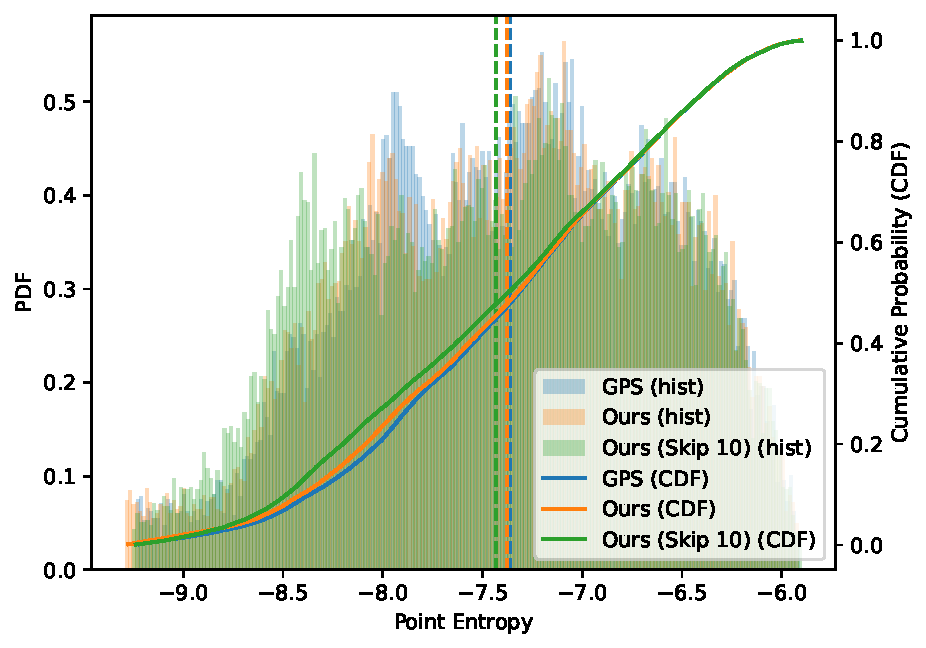
\includegraphics[width=0.45\linewidth]{images/map_eval/entropy_gps_ours_skip_3000--50.pdf}
    }
    \subcaptionbox{Output point cloud. Points are colored by height.}{
        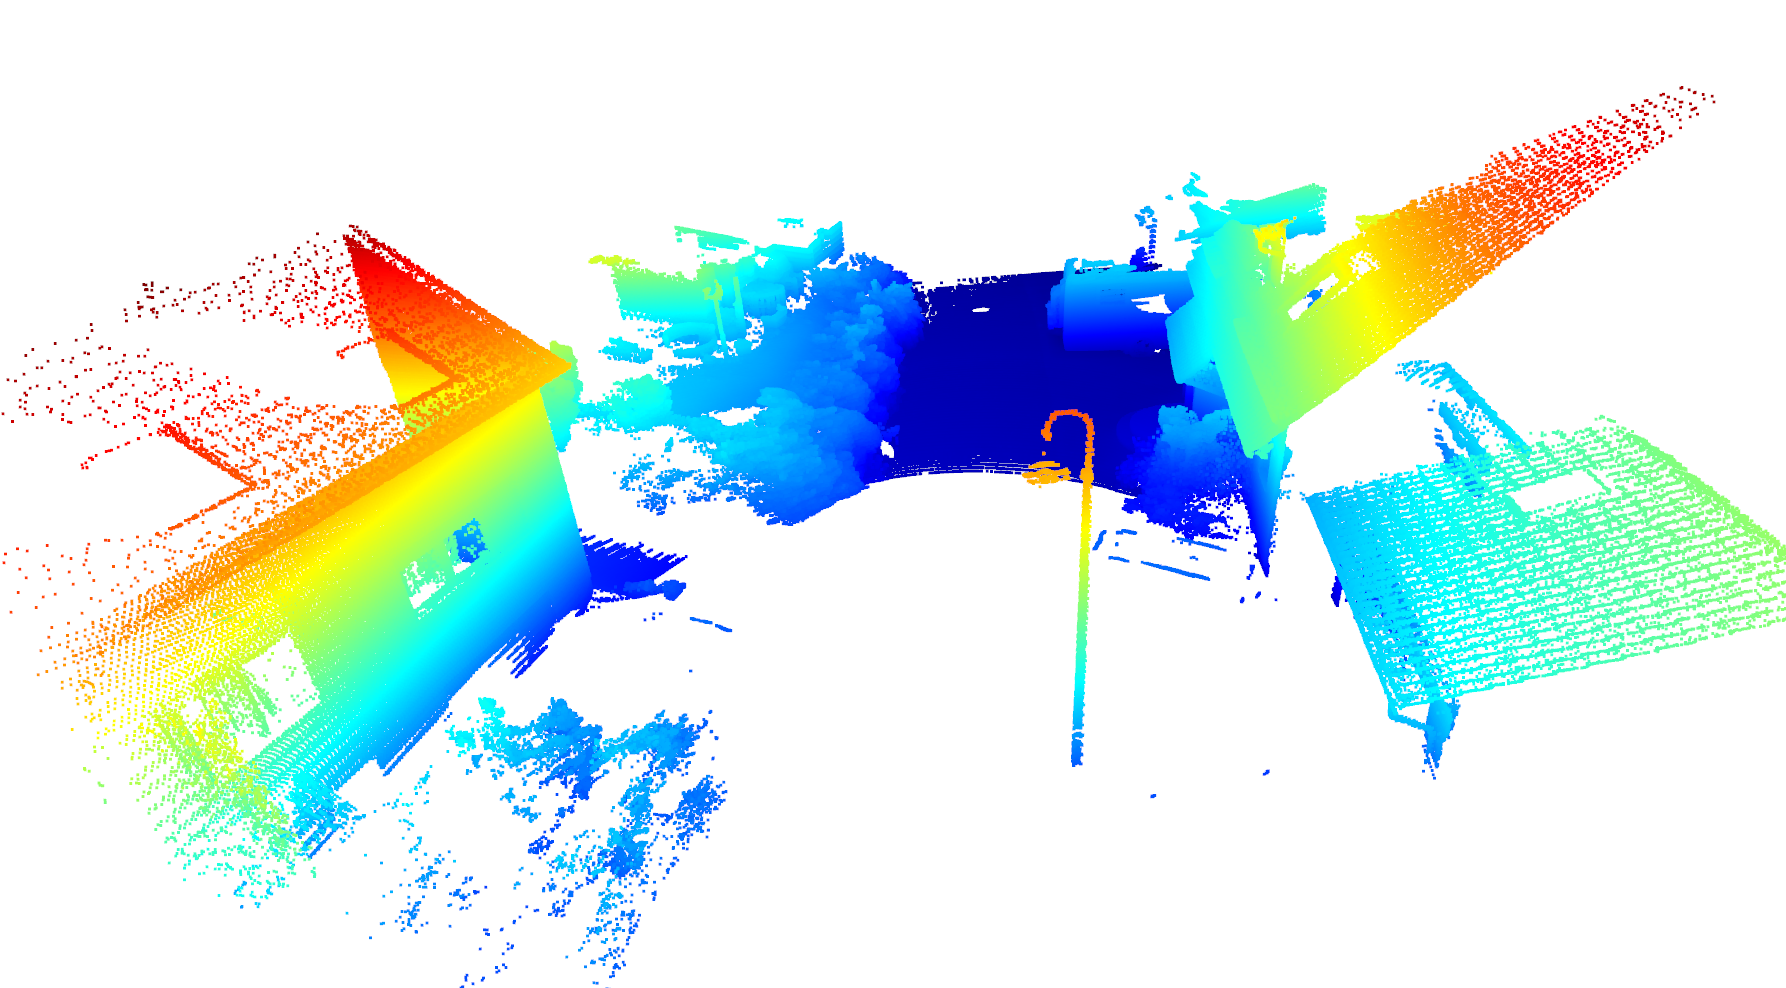
\includegraphics[width=0.5\linewidth]{images/map_eval/viz-3000--50.png}
    }
    \caption[Map comparison in a rural scene]{Map evaluation in a rural street scene, built from 50 consecutive scans. Point entropy is decreased, indicating better mapping.}
    \label{fig:map-eval-regular}
\end{figure}
\begin{figure}[h]
    \centering
    \subcaptionbox{Point entropy comparison. Dashed line indicates median value of each distribution.}{
        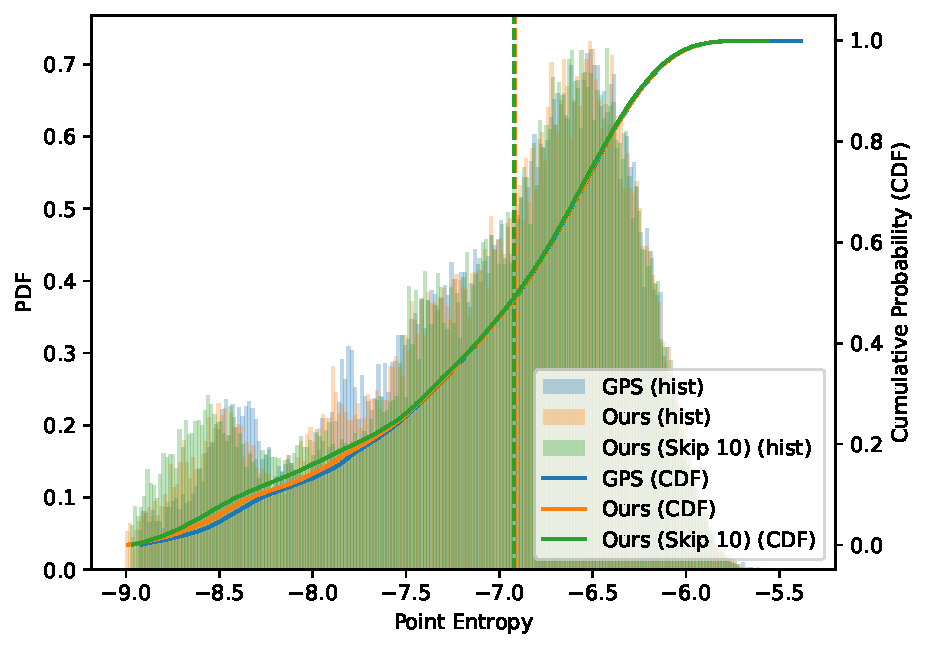
\includegraphics[width=0.45\linewidth]{images/map_eval/entropy_gps_ours_skip-200--50.pdf}
    }
    \subcaptionbox{Output point cloud. Points are colored by height.}{
        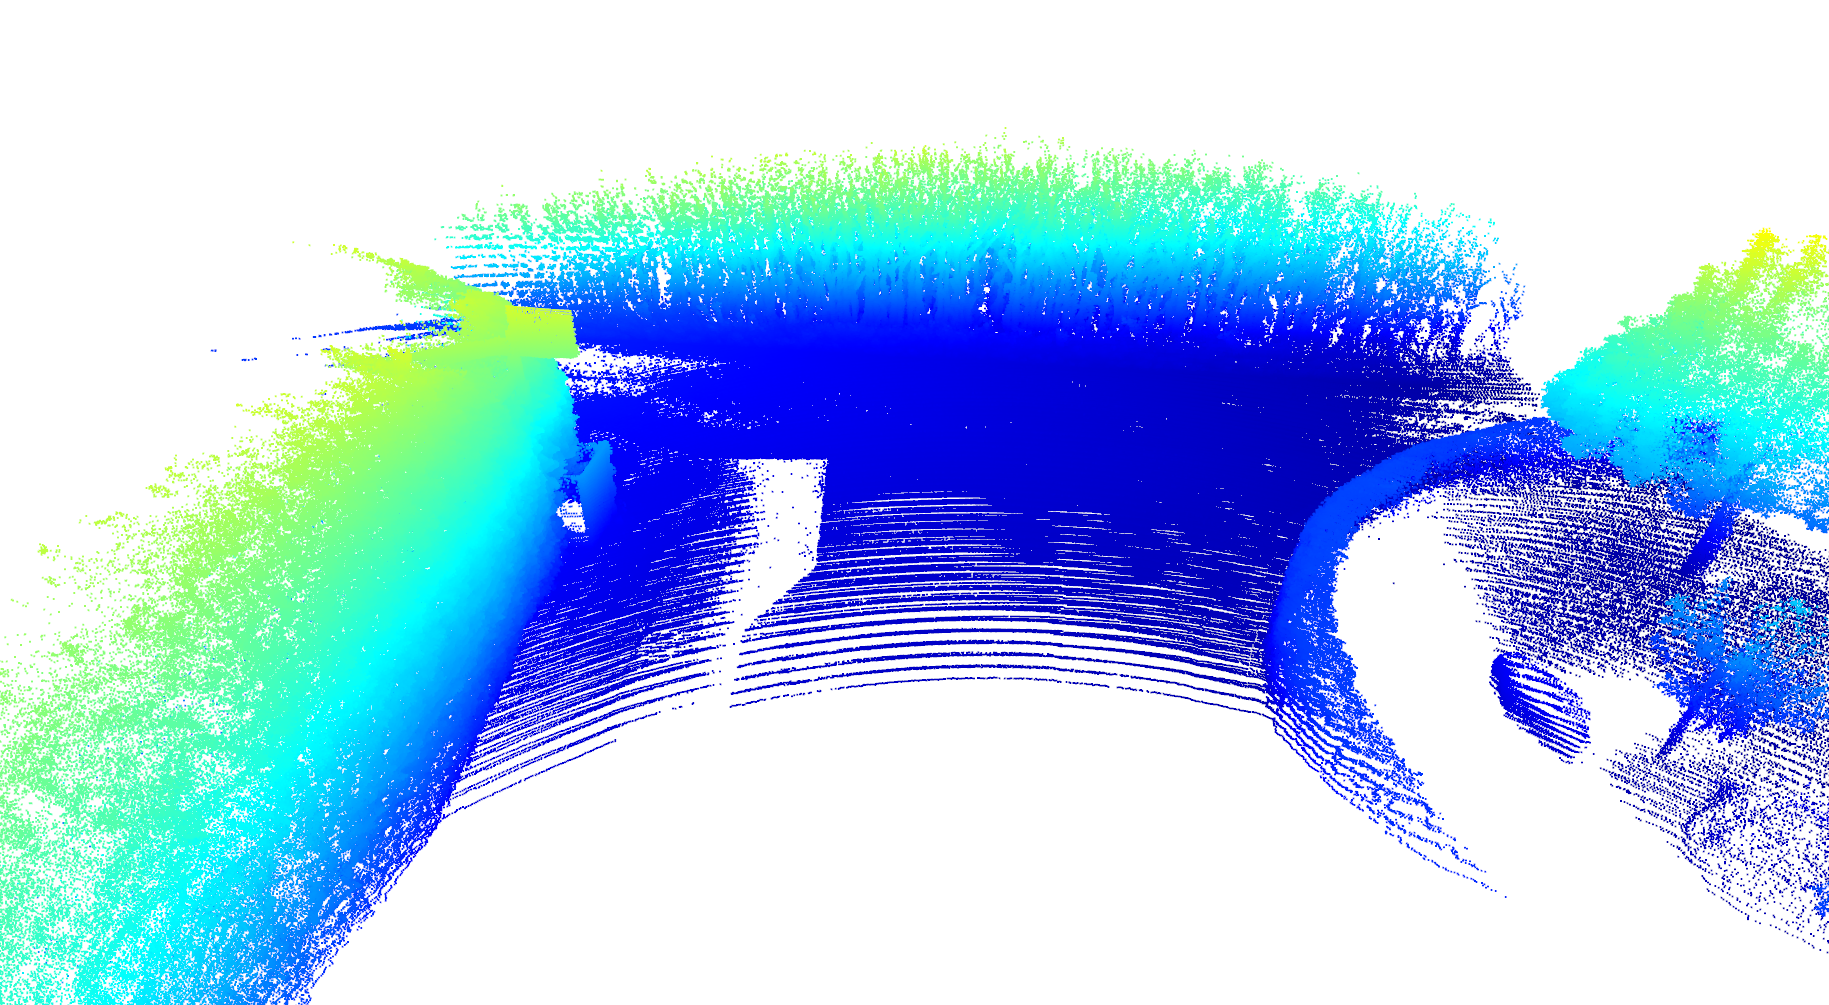
\includegraphics[width=0.5\linewidth]{images/map_eval/viz-200--50.png}
    }
    \caption[Map comparison in a vegetation-dominated scene]{Map evaluation in a vegetation-dominated scene, built from 50 consecutive scans. Point entropy is decreased, indicating better mapping.}
    \label{fig:map-eval-vegetation}
\end{figure}



% Point entropy comparison - OK
% Point to plane error comparison - 
% Nearest neighbor distance comparison - Not a big difference

% Visual analysis

% Scan to scan RMSE 
% Consecutive, every 2, every 3?


% Scan to map RMSE
% create map from surrounding poses, check middle scan

% \section{KITTI results}

% Things worth mentioning
% - execution time
\cleardoublepage

\chapter{Conclusion}
\label{ch:conclusion}

This work addressed odometry, a fundamental topic of mobile robotics, with emphasis on the area of perception, and was driven by its applicability to an industrial product, the SDX-Compact manufactured by Sodex Innovations GmbH. Range information from a 360-degree LiDAR sensor is fused with localization and orientation measurements provided by an INS, to increase robustness to GPS perturbations and enable 3D mapping quality beyond the accuracy of RTK-corrected readings.

We provided a review of the current state of research around this problem and its many facets. This was followed by a presentation of the hardware and data that we operate on, and a detailed explanation of the experiments conducted around each component of our final solution. Our contribution is an original displacement estimation method which relies on a two-step scan alignment process (robust ICP and Generalized ICP) and a factor graph structure, for integrating GPS readings. To enforce point cloud registration constraints, we add ``skip connections'' between non-consecutive poses, based on the ICP-estimated displacement.

% discuss results
% discuss general conclusions about the data used and the problems encountered

% \section{Future Work}
% Z drift
% integrate RGB data
% improve performance
\cleardoublepage

% \input{samples_en/intro.tex}
% \cleardoublepage

% \chapter{User documentation}
\label{ch:user}

Lorem ipsum dolor sit amet $\mathbb{N}$\nomenclature{$\mathbb{N}$}{Set of natural numbers}, consectetur adipiscing elit. Duis nibh leo, dapibus in elementum nec, aliquet id sem. Suspendisse potenti. Nullam sit amet consectetur nibh. Donec scelerisque varius turpis at tincidunt. Cras a diam in mauris viverra vehicula. Vivamus mi odio, fermentum vel arcu efficitur, lacinia viverra nibh. Aliquam aliquam ante mi, vel pretium arcu dapibus eu. Nulla finibus ante vel arcu tincidunt, ut consectetur ligula finibus. Mauris mollis lectus sed ipsum bibendum, ac ultrices erat dictum. Suspendisse faucibus euismod lacinia $\mathbb{Z}$\nomenclature{$\mathbb{Z}$}{Set of integer numbers}.


\section{Enumerations and lists}

Etiam vel odio ante. Etiam pulvinar nibh quis massa auctor congue. Pellentesque quis odio vitae sapien molestie vestibulum sit amet et quam. Pellentesque vel dui eget enim hendrerit finibus at sit amet libero. Quisque sollicitudin ultrices enim, nec porta magna imperdiet vitae. Cras condimentum nunc dui, eget molestie nunc accumsan vel.

\begin{itemize}
	\item Fusce in aliquet neque, in pretium sem.
	\item Donec tincidunt tellus id lectus pretium fringilla.
	\item Nunc faucibus, erat pretium tempus tempor, tortor mi fringilla neque, ac congue ex dui vitae mauris.
\end{itemize}

Donec dapibus sodales ante, at scelerisque nunc laoreet sit amet. Mauris porttitor tincidunt neque, vel ullamcorper neque pulvinar et. Integer eu lorem euismod, faucibus lectus sed, accumsan felis. Nunc ornare mi at augue vulputate, eu venenatis magna mollis. Nunc sed posuere dui, et varius nulla. Sed mollis nibh augue, eget scelerisque eros ornare nec.

\begin{enumerate}
	\item\label{step:first} Donec pretium et quam a cursus. Ut sollicitudin tempus urna et mollis.
	\item Aliquam et aliquam turpis, sed fermentum mauris. Nulla eget ex diam.
	\item Donec eget tellus pharetra, semper neque eget, rutrum diam Step~\ref{step:first}.
\end{enumerate}

Praesent porta, metus eget eleifend consequat, eros ligula eleifend ex, a pellentesque mi est vitae urna. Vivamus turpis nunc, iaculis non leo eget, mattis vulputate tellus. Maecenas rutrum eros sem, pharetra interdum nulla porttitor sit amet. In vitae viverra ante. Maecenas sit amet placerat orci, sed tincidunt velit. Vivamus mattis, enim vel suscipit elementum, quam odio venenatis elit\footnote{Phasellus faucibus varius purus, nec tristique enim porta vitae.}, et mollis nulla nunc a risus. Praesent purus magna, tristique sed lacus sit amet, convallis malesuada magna. 

\begin{description}
	\item[Vestibulum venenatis] malesuada enim, ac auctor erat vestibulum et. Phasellus id purus a leo suscipit accumsan.
	\item[Orci varius natoque] penatibus et magnis dis parturient montes, nascetur ridiculus mus. Nullam interdum rhoncus nisl, vel pharetra arcu euismod sagittis. Vestibulum ac turpis auctor, viverra turpis at, tempus tellus.
	\item[Morbi dignissim] erat ut rutrum aliquet. Nulla eu rutrum urna. Integer non urna at mauris scelerisque rutrum sed non turpis.
\end{description}

\subsection{Lists with narrow spacing inbetween items}

Phasellus ultricies, sapien sit amet ultricies placerat, velit purus viverra ligula, id consequat ipsum odio imperdiet enim:
\begin{compactenum}
	\item Maecenas eget lobortis leo.
	\item Donec eget libero enim.
	\item In eu eros a eros lacinia maximus ullamcorper eget augue.
\end{compactenum}

\bigskip

In quis turpis metus. Proin maximus nibh et massa eleifend, a feugiat augue porta. Sed eget est purus. Duis in placerat leo. Donec pharetra eros nec enim convallis:
\begin{compactitem}
	\item Pellentesque odio lacus.
	\item Maximus ut nisl auctor.
	\item Sagittis vulputate lorem.
\end{compactitem}

\bigskip

Vestibulum ante ipsum primis in faucibus orci luctus et ultrices posuere cubilia Curae; Sed lorem libero, dignissim vitae gravida a, ornare vitae est.
\begin{compactdesc}
	\item[Cras maximus] massa commodo pellentesque viverra.
	\item[Morbi sit] amet ante risus. Aliquam nec sollicitudin mauris
	\item[Ut aliquam rhoncus sapien] luctus viverra arcu iaculis posuere
\end{compactdesc}


\section{Images and figures}

Aliquam vehicula luctus mi a pretium. Nulla quam neque, maximus nec velit in, aliquam mollis tortor. Aliquam erat volutpat. Curabitur vitae laoreet turpis. Integer id diam ligula. Nulla sodales purus id mi consequat, eu venenatis odio pharetra. Cras a arcu quam. Suspendisse augue risus, pulvinar a turpis et, commodo aliquet turpis. Nulla aliquam scelerisque mi eget pharetra. Mauris sed posuere elit, ac lobortis metus. Proin lacinia sit amet diam sed auctor. Nam viverra orci id sapien sollicitudin, a aliquam lacus suscipit, Figure~\ref{fig:example-1}:

\begin{figure}[H]
	\centering
	
\includegraphics[width=0.6\textwidth,height=100px]{elte_cimer_szines}
	\caption{Quisque ac tincidunt leo}
	\label{fig:example-1}
\end{figure}

\subsection{Framing figures}

Ut aliquet nec neque eget fermentum. Cras volutpat tellus sed placerat elementum. Quisque neque dui, consectetur nec finibus eget, blandit id purus. Nam eget ipsum non nunc placerat interdum.

\begin{figure}[H]
	\centering
	
\includegraphics[width=0.6\textwidth,height=100px,frame]{elte_cimer_szines}
	\caption{Quisque ac tincidunt leo}
\end{figure}

\subsection{Subfigures}

In non ipsum fermentum urna feugiat rutrum a at odio. Pellentesque habitant morbi tristique senectus et netus et malesuada fames ac turpis egestas. Nulla tincidunt mattis nisl id suscipit. Sed bibendum ac felis sed volutpat. Nam pharetra nisi nec facilisis faucibus. Aenean tristique nec libero non commodo. Nulla egestas laoreet tempus. Nunc eu aliquet nulla, quis vehicula dui. Proin ac risus sodales, gravida nisi vitae, efficitur neque, Figure~\ref{fig:example-2}:

\begin{figure}[H]
	\centering
	\subcaptionbox{Vestibulum quis mattis urna}{
		
\includegraphics[width=0.45\linewidth]{elte_cimer_szines}}
	\hspace{5pt}
	\subcaptionbox{Donec hendrerit quis dui sit amet venenatis}{
		
\includegraphics[width=0.45\linewidth]{elte_cimer_szines}}
	\caption{Aenean porttitor mi volutpat massa gravida}
	\label{fig:example-2}
\end{figure}

Nam et nunc eget elit tincidunt sollicitudin. Quisque ligula ipsum, tempor vitae tortor ut, commodo rhoncus diam. Pellentesque habitant morbi tristique senectus et netus et malesuada fames ac turpis egestas. Phasellus vehicula quam dui, eu convallis metus porta ac.


\section{Tables}

Nam magna ex, euismod nec interdum sed, sagittis nec leo. Nam blandit massa bibendum mattis tristique. Phasellus tortor ligula, sodales a consectetur vitae, placerat vitae dolor. Aenean consequat in quam ac mollis. 

\begin{table}[H]
	\centering
	\begin{tabular}{ | m{0.25\textwidth} | m{0.65\textwidth} | }
		\hline
		\textbf{Phasellus tortor} & \textbf{Aenean consequat} \\
		\hline \hline
		\emph{Sed malesuada} & Aliquam aliquam velit in convallis ultrices. \\
		\hline
		\emph{Purus sagittis} &  Quisque lobortis eros vitae urna lacinia euismod. \\
		\hline
		\emph{Pellentesque} & Curabitur ac lacus pellentesque, eleifend sem ut, placerat enim. Ut auctor tempor odio ut dapibus. \\
		\hline
	\end{tabular}
	\caption{Maecenas tincidunt non justo quis accumsan}
	\label{tab:example-1}
\end{table}

\subsection{Multi rows and multi columns}

Mauris a dapibus lectus. Vestibulum commodo nibh ante, ut maximus magna eleifend vel. Integer vehicula elit non lacus lacinia, vitae porttitor dolor ultrices. Vivamus gravida faucibus efficitur. Ut non erat quis arcu vehicula lacinia. Nulla felis mauris, laoreet sed malesuada in, euismod et lacus. Aenean at finibus ipsum. Pellentesque dignissim elit sit amet lacus congue vulputate.

\begin{table}[htb]
	\centering
	\begin{tabular}{ | c | r | r | r | r | r | r | }
		\hline
		\multirow{2}{*}{\textbf{Quisque}} & \multicolumn{2}{ c | }{\textbf{Suspendisse}} & \multicolumn{2}{ c | }{\textbf{Aliquam}} & \multicolumn{2}{ c | }{\textbf{Vivamus}} \\
		\cline{2-7}
		& Proin & Nunc & Proin & Nunc & Proin & Nunc \\
		\hline \hline		
		Leo & 2,80 MB & 100\% & 232 KB & 8,09\% & 248 KB & 8,64\% \\
		\hline
		Vel & 9,60 MB & 100\% & 564 KB & 5,74\% & 292 KB & 2,97\% \\
		\hline
		Auge & 78,2 MB & 100\% & 52,3 MB & 66,88\% & 3,22 MB & 4,12\% \\
		\hline 
	\end{tabular}
	\caption[Rövid cím a táblázatjegyzékbe]{Vivamus ac arcu fringilla, fermentum neque sed, interdum erat. Mauris bibendum mauris vitae enim mollis, et eleifend turpis aliquet.}
	\label{tab:example-2}
\end{table}

\subsection{Long tables over multiple pages}

Nunc porta placerat leo, sit amet porttitor dui porta molestie. Aliquam at fermentum mi. Maecenas vitae lorem at leo tincidunt volutpat at nec tortor. Vivamus semper lacus eu diam laoreet congue. Vivamus in ipsum risus. Nulla ullamcorper finibus mauris non aliquet. Vivamus elementum rhoncus ex ut porttitor.

\begin{center}
	\begin{longtable}{ | p{0.3\textwidth} | p{0.7\textwidth} | }
		
		\hline
		\multicolumn{2}{|c|}{\textbf{Praesent aliquam mauris enim}}
		\\ \hline
		
		\emph{Suspendisse potenti} & \emph{Lorem ipsum dolor sit amet}
		\\ \hline \hline
		\endfirsthead % table header on first page
		
		\hline
		\emph{Suspendisse potenti} & \emph{Lorem ipsum dolor sit amet}
		\\ \hline \hline
		\endhead % table header on further pages
		
		\hline
		\endfoot % table footer on previous pages
		
		\endlastfoot % table footer on last page
		
		\emph{Praesent}
		& Nulla ultrices et libero sit amet fringilla. Nunc scelerisque ante tempus sapien placerat convallis.
		\\ \hline
		
		\emph{Luctus}
		& Integer hendrerit erat massa, non hendrerit risus convallis at. Curabitur ultrices, justo in imperdiet condimentum, neque tortor luctus enim, luctus posuere massa erat vitae nibh.
		\\ \hline
		
		\emph{Egestas}
		& Duis fermentum feugiat augue in blandit. Mauris a tempor felis. Pellentesque ultricies tristique dignissim. Pellentesque aliquam semper tristique. Nam nec egestas dolor. Vestibulum id elit quis enim fringilla tempor eu a mauris. Aliquam vitae lacus tellus. Phasellus mauris lectus, aliquam id leo eget, auctor dapibus magna. Fusce lacinia felis ac elit luctus luctus.
		\\ \hline
		
		\emph{Dignissim}
		& Praesent aliquam mauris enim, vestibulum posuere massa facilisis in. Suspendisse potenti. Nam quam purus, rutrum eu augue ut, varius vehicula tellus. Fusce dui diam, aliquet sit amet eros at, sollicitudin facilisis quam. Phasellus tempor metus vel augue gravida pretium. Proin aliquam aliquam blandit. Nulla id tempus mi. Fusce in aliquam tortor.
		\\ \hline
		
		\emph{Pellentesque}
		& Donec felis nibh, imperdiet a arcu non, vehicula gravida nibh. Quisque interdum sapien eu massa commodo, ac elementum felis faucibus.
		\\ \hline
		
		\emph{Molestie}
		& Cras ullamcorper tellus et auctor ultricies. Maecenas tincidunt euismod lectus nec venenatis. Suspendisse potenti. Pellentesque pretium nunc ut euismod cursus. Nam venenatis condimentum quam. Curabitur suscipit efficitur aliquet. Interdum et malesuada fames ac ante ipsum primis in faucibus.
		\\ \hline
		
		\emph{Vivamus semper}
		& In purus purus, faucibus eu libero vulputate, tristique sodales nunc. Nulla ut gravida dolor. Fusce vel pellentesque mi, vel efficitur eros. Nunc vitae elit tellus. Sed vestibulum auctor consequat. 
		\\ \hline
		
		\emph{Condimentum}
		& Nulla scelerisque, leo et facilisis pretium, risus enim cursus turpis, eu suscipit ipsum ipsum in mauris. Praesent eget pulvinar ipsum, suscipit interdum nunc. Nam varius massa ut justo ullamcorper sollicitudin. Vivamus facilisis suscipit neque, eu fermentum risus. Ut at mi mauris.
		\\ \hline
		
		\caption{Praesent ullamcorper consequat tellus ut eleifend}
		\label{tab:example-3}		
	\end{longtable}
\end{center}
% \cleardoublepage

% \chapter{Developer documentation}
\label{ch:impl}

Lorem ipsum dolor sit amet, consectetur adipiscing elit. Duis nibh leo, dapibus in elementum nec, aliquet id sem. Suspendisse potenti. Nullam sit amet consectetur nibh. Donec scelerisque varius turpis at tincidunt.


\section{Theorem-like environments}

\begin{definition}
Mauris tristique sollicitudin ultrices. Etiam tristique quam sit amet metus dictum imperdiet. Nunc id lorem sed nisl pulvinar aliquet vitae quis arcu. Morbi iaculis eleifend porttitor.
\end{definition}

Maecenas rutrum eros sem, pharetra interdum nulla porttitor sit amet. In vitae viverra ante. Maecenas sit amet placerat orci, sed tincidunt velit. Vivamus mattis, enim vel suscipit elementum, quam odio venenatis elit, et mollis nulla nunc a risus. Praesent purus magna, tristique sed lacus sit amet, convallis malesuada magna. Phasellus faucibus varius purus, nec tristique enim porta vitae.

\begin{theorem}
Nulla finibus ante vel arcu tincidunt, ut consectetur ligula finibus. Mauris mollis lectus sed ipsum bibendum, ac ultrices erat dictum. Suspendisse faucibus euismod lacinia. Etiam vel odio ante.
\end{theorem}
\begin{proof}
Etiam pulvinar nibh quis massa auctor congue. Pellentesque quis odio vitae sapien molestie vestibulum sit amet et quam. Pellentesque vel dui eget enim hendrerit finibus at sit amet libero. Quisque sollicitudin ultrices enim, nec porta magna imperdiet vitae. Cras condimentum nunc dui.
\end{proof}

Donec dapibus sodales ante, at scelerisque nunc laoreet sit amet. Mauris porttitor tincidunt neque, vel ullamcorper neque pulvinar et. Integer eu lorem euismod, faucibus lectus sed, accumsan felis. 

\begin{remark}
Nunc ornare mi at augue vulputate, eu venenatis magna mollis. Nunc sed posuere dui, et varius nulla. Sed mollis nibh augue, eget scelerisque eros ornare nec. Praesent porta, metus eget eleifend consequat, eros ligula eleifend ex, a pellentesque mi est vitae urna. Vivamus turpis nunc, iaculis non leo eget, mattis vulputate tellus.
\end{remark}

Fusce in aliquet neque, in pretium sem. Donec tincidunt tellus id lectus pretium fringilla. Nunc faucibus, erat pretium tempus tempor, tortor mi fringilla neque, ac congue ex dui vitae mauris. Donec pretium et quam a cursus.

\begin{note}
Aliquam vehicula luctus mi a pretium. Nulla quam neque, maximus nec velit in, aliquam mollis tortor. Aliquam erat volutpat. Curabitur vitae laoreet turpis. Integer id diam ligula.
\end{note}

Ut sollicitudin tempus urna et mollis. Aliquam et aliquam turpis, sed fermentum mauris. Nulla eget ex diam. Donec eget tellus pharetra, semper neque eget, rutrum diam.

\subsection{Equations, formulas}

Duis suscipit ipsum nec urna blandit, $2 + 2 = 4$ pellentesque vehicula quam fringilla. Vivamus euismod, lectus sit amet euismod viverra, dolor metus consequat sapien, ut hendrerit nisl nulla id nisi. Nam in leo eu quam sollicitudin semper a quis velit.

$$a^2 + b^2 = c^2$$

Phasellus mollis, elit sed convallis feugiat, dolor quam dapibus nibh, suscipit consectetur lacus risus quis sem. Vivamus scelerisque porta odio, vitae euismod dolor accumsan ut.

In mathematica, identitatem Euleri (equation est scriptor vti etiam notum) sit aequalitatem Equation~\ref{eq:euler}:
\begin{equation}\label{eq:euler}
e^{i \times \pi} + 1 = 0
\end{equation}

Vestibulum ante ipsum primis in faucibus orci luctus et ultrices posuere cubilia curae; Nullam pulvinar purus at pharetra elementum.
Aequationes adsignans aequationis signum:
\begin{align}
	A & = \frac{\pi r^2}{2} \\
	& = \frac{1}{2} \pi r^2
\end{align}

Proin tempor risus a efficitur condimentum. Cras lobortis ligula non sollicitudin euismod. Fusce non pellentesque nibh, non elementum tellus.
Omissa numeratione aliquarum aequationum:
\begin{align}
	f(u) & =\sum_{j=1}^{n} x_jf(u_j) \nonumber \\
	& =\sum_{j=1}^{n} x_j \sum_{i=1}^{m} a_{ij}v_i \nonumber \\
	& =\sum_{j=1}^{n} \sum_{i=1}^{m} a_{ij}x_jv_i
\end{align}

\section{Source code samples}

Nulla sodales purus id mi consequat, eu venenatis odio pharetra. Cras a arcu quam. Suspendisse augue risus, pulvinar a turpis et, commodo aliquet turpis. Nulla aliquam scelerisque mi eget pharetra. Mauris sed posuere elit, ac lobortis metus. Proin lacinia sit amet diam sed auctor. Nam viverra orci id sapien sollicitudin, a aliquam lacus suscipit. Quisque ac tincidunt leo Code~\ref{src:cpp} and \ref{src:csharp}:

\lstset{caption={Hello World in C++}, label=src:cpp}
\begin{lstlisting}[language={C++}]
#include <stdio>

int main() 
{
	int c;
	std::cout << "Hello World!" << std::endl;

	std::cout << "Press any key to exit." << std::endl;
	std::cin >> c;
	
	return 0;
}
\end{lstlisting}

\lstset{caption={Hello World in C\#}, label=src:csharp}
\begin{lstlisting}[language={[Sharp]C}]
using System;
namespace HelloWorld
{
	class Hello 
	{
		static void Main() 
		{
			Console.WriteLine("Hello World!");
			
			Console.WriteLine("Press any key to exit.");
			Console.ReadKey();
		}
	}
}
\end{lstlisting}

\subsection{Algorithms}

A general Interval Branch and Bound algorithm is shown in Algorithm~\ref{alg:ibb}. An appropriate selection rule is applied in Step~\ref{step:selrule}.\\
Source of example: \href{https://www.inf.u-szeged.hu/actacybernetica/}{Acta Cybernetica (this is a hyperlink)}.

\begin{algorithm}[H]
\caption{A general interval B\&B algorithm} 
\label{alg:ibb} 
\textbf{\underline{Funct}} IBB($S,f$)
\begin{algorithmic}[1] % display line numbers before every n line, here n = 1
\State Set the working list ${\cal L}_W$ := $\{S\}$ and the final list ${\cal L}_Q$ := $\{\}$     
\While{( ${\cal L}_W \neq \emptyset$ )} \label{alg:igoend}
	\State  Select an interval $X$ from ${\cal L}_W$ \label{step:selrule}\Comment{Selection rule}  
	\State Compute $lbf(X)$ \Comment{Bounding rule}		  
	\If{$X$ cannot be eliminated} \Comment{Elimination rule}
		\State Divide $X$ into $X^j,\ j=1,\dots, p$, subintervals   \Comment{Division rule}
		\For{$j=1,\ldots,p$}
			\If{$X^j$ satisfies the termination criterion} \Comment{Termination rule}
				\State Store $X^j$ in ${\cal L}_W$ 
			\Else
				\State Store $X^j$ in ${\cal L}_W$ 
			\EndIf
		\EndFor  
	\EndIf
\EndWhile
\State \textbf{return} ${\cal L}_Q$
\end{algorithmic}
\end{algorithm}

% \cleardoublepage

% \input{samples_en/sum.tex}
% \cleardoublepage

% Acknowledgements (optional) - in case your thesis received funding or would like to express special thanks to someone
% \chapter*{\acklabel}
% \addcontentsline{toc}{chapter}{\acklabel}
% In case your thesis received financial support from a project or the university, it is usually required to indicate the proper attribution in the thesis itself. Special thanks can also be expressed towards teachers, fellow students and colleagues who helped you in the process of creating your thesis.

% Appendices (optional) - useful for detailed information in long tables, many and/or large figures, etc.
% \appendix
% \chapter{Simulation results}
\label{appx:simulation}

Lorem ipsum dolor sit amet, consectetur adipiscing elit. Pellentesque facilisis in nibh auctor molestie. Donec porta tortor mauris. Cras in lacus in purus ultricies blandit. Proin dolor erat, pulvinar posuere orci ac, eleifend ultrices libero. Donec elementum et elit a ullamcorper. Nunc tincidunt, lorem et consectetur tincidunt, ante sapien scelerisque neque, eu bibendum felis augue non est. Maecenas nibh arcu, ultrices et libero id, egestas tempus mauris. Etiam iaculis dui nec augue venenatis, fermentum posuere justo congue. Nullam sit amet porttitor sem, at porttitor augue. Proin bibendum justo at ornare efficitur. Donec tempor turpis ligula, vitae viverra felis finibus eu. Curabitur sed libero ac urna condimentum gravida. Donec tincidunt neque sit amet neque luctus auctor vel eget tortor. Integer dignissim, urna ut lobortis volutpat, justo nunc convallis diam, sit amet vulputate erat eros eu velit. Mauris porttitor dictum ante, commodo facilisis ex suscipit sed.

Sed egestas dapibus nisl, vitae fringilla justo. Donec eget condimentum lectus, molestie mattis nunc. Nulla ac faucibus dui. Nullam a congue erat. Ut accumsan sed sapien quis porttitor. Ut pellentesque, est ac posuere pulvinar, tortor mauris fermentum nulla, sit amet fringilla sapien sapien quis velit. Integer accumsan placerat lorem, eu aliquam urna consectetur eget. In ligula orci, dignissim sed consequat ac, porta at metus. Phasellus ipsum tellus, molestie ut lacus tempus, rutrum convallis elit. Suspendisse arcu orci, luctus vitae ultricies quis, bibendum sed elit. Vivamus at sem maximus leo placerat gravida semper vel mi. Etiam hendrerit sed massa ut lacinia. Morbi varius libero odio, sit amet auctor nunc interdum sit amet.

Aenean non mauris accumsan, rutrum nisi non, porttitor enim. Maecenas vel tortor ex. Proin vulputate tellus luctus egestas fermentum. In nec lobortis risus, sit amet tincidunt purus. Nam id turpis venenatis, vehicula nisl sed, ultricies nibh. Suspendisse in libero nec nisi tempor vestibulum. Integer eu dui congue enim venenatis lobortis. Donec sed elementum nunc. Nulla facilisi. Maecenas cursus id lorem et finibus. Sed fermentum molestie erat, nec tempor lorem facilisis cursus. In vel nulla id orci fringilla facilisis. Cras non bibendum odio, ac vestibulum ex. Donec turpis urna, tincidunt ut mi eu, finibus facilisis lorem. Praesent posuere nisl nec dui accumsan, sed interdum odio malesuada.
% \cleardoublepage


% Bibliography (mandatory)
\phantomsection
\addcontentsline{toc}{chapter}{\biblabel}
\printbibliography[title=\biblabel]
\cleardoublepage

% List of figures (optional) - useful over 3-5 figures
\phantomsection
\addcontentsline{toc}{chapter}{\lstfigurelabel}
\listoffigures
\cleardoublepage

% List of tables (optional) - useful over 3-5 tables
% \phantomsection
% \addcontentsline{toc}{chapter}{\lsttablelabel}
% \listoftables
% \cleardoublepage

% List of algorithms (optional) - useful over 3-5 algorithms
% \phantomsection
% \addcontentsline{toc}{chapter}{\lstalgorithmlabel}
% \listofalgorithms
% \cleardoublepage

% List of codes (optional) - useful over 3-5 code samples
% \phantomsection
% \addcontentsline{toc}{chapter}{\lstcodelabel}
% \lstlistoflistings
% \cleardoublepage

% List of symbols (optional)
%\printnomenclature

{\setlength{\baselineskip}{0.6\baselineskip} % Adjust 0.9 to reduce spacing
    \printglossary[type=\acronymtype]
    \printglossary
}

\end{document}
